%==============================================================================
% Importando a classe
%==============================================================================
\documentclass{templufla}          

%==============================================================================
% Pacote hyperref para referências cruzadas dentro do documento \ref e \autoref
% O pacote hyperref precisa ser importado o mais cedo possível.

% Setspace precisa estar antes do hyperref para usar a versão atual do abntex.
\usepackage{setspace}

% Definindo cores para os links cruzados
\usepackage{xcolor}              % para mais cores
\definecolor{rltred}{rgb}{0.2,0,0}
\definecolor{rltgreen}{rgb}{0,0.2,0}
\definecolor{rltblue}{rgb}{0,0,0.2}


% Importa hyperref
\usepackage[%
hidelinks, % colorlinks=true, | Troque se quiser link com cor
urlcolor=rltblue,       % \href{...}{...} external (URL)
filecolor=rltgreen,     % \href{...} local file
linkcolor=rltred,       % \ref{...} and \pageref{...}
citecolor=rltgreen,%
]{hyperref} % 


%==============================================================================
% Configurando a linguagem do template

% Português
\usepackage[english,brazilian]{babel}
% Adaptando os nomes das seções
\addto\captionsbrazil{
	\renewcommand{\chaptername}{Seção}
	\renewcommand{\subsectionname}{Seção}
	\renewcommand{\subsubsectionname}{Seção}
}
\addto\extrasbrazil{
	\renewcommand{\chapterautorefname}{Seção}
	\renewcommand{\subsectionautorefname}{Seção}
	\renewcommand{\subsubsectionautorefname}{Seção}
}

% Inglês
%\usepackage[english]{babel}
%% Adapta nomes de seção
\addto\captionsenglish{
	\renewcommand{\chaptername}{Section}
	\renewcommand{\subsectionname}{Section}
	\renewcommand{\subsubsectionname}{Section}
}
\addto\extrasenglish{
	\renewcommand{\chapterautorefname}{Section}
	\renewcommand{\subsectionautorefname}{Section}
	\renewcommand{\subsubsectionautorefname}{Section}
}

% Adaptar nomes fixos

% títulos de pessoa
\renewcommand{\orientadorname}{Advisor}
\renewcommand{\orientadoraname}{Advisor}
\renewcommand{\coorientadorname}{Co-advisor}
\renewcommand{\coorientadoraname}{Co-advisor}

% títulos
\renewcommand{\agradecimentosname}{Acknowledgments}
\renewcommand{\listadefigurasname}{List of Figures}
\renewcommand{\listadeilustracoesname}{List of Illustrations}
\renewcommand{\listadegraficosname}{List of Plots}
\renewcommand{\listadetabelasname}{List of Tables}
\renewcommand{\listadequadrosname}{List of Frames}
\renewcommand{\listadeexemplosname}{List of Examples}
\renewcommand{\listadeteoremasname}{List of Theorems}
\renewcommand{\listadeabreviaturasname}{List of Abbreviations}
\renewcommand{\listadesiglasname}{List of Acronyms}
\renewcommand{\listadesimbolosname}{List of Symbols}
\renewcommand{\referenciasname}{References}
\renewcommand{\glossarioname}{Glossary}
\renewcommand{\anexosname}{Annexes}
\renewcommand{\apendicesname}{Appendixes}
\renewcommand{\indicename}{Index}


% elementos
\renewcommand{\ilustracaoname}{Illustration}
\renewcommand{\graficoname}{Plot}
\renewcommand{\quadroname}{Frame}
\renewcommand{\exemploname}{Example}
\renewcommand{\teoremaname}{Theorem}
\renewcommand{\anexoname}{Annex}
\renewcommand{\apendicename}{Appendix}

% geral
\renewcommand{\fontename}{Source}
\renewcommand{\aprovadaemname}{ACCEPTED on }

%==============================================================================
% Configuração dos pacotes necessários
% Primeiros pacotes (alguns precisam ser importados depois)

% TEXTOS
\usepackage[T1]{fontenc}         % usa fontes postscript com acentos
\usepackage[utf8]{inputenc}      % permite edição direta com acentos
\usepackage{listings}            % para inserção de código
\usepackage{fancyvrb}            % para inserção de saídas de comandos

% MATEMÁTICA
\usepackage{amsmath}             % pacote da AMS para Matemática Avançada
\usepackage{amssymb}             % símbolos extras da AMS
\usepackage{mathtools}			 % para mais comandos de matemática
\usepackage{latexsym}            % símbolos extras do LaTeX

% TABELAS
\usepackage{longtable}           % para tabelas muito grandes
\usepackage{array}               % para mais opções em tabelas
\usepackage{colortbl}            % para cores em tabelas
\usepackage{multirow}            % para células com várias linhas
\usepackage{multicol}            % para células com várias colunas

% FIGUAS E GRÁFICOS
\usepackage{subfigure}           % para figuras dentro de figuras
\usepackage{caption}             % para remodelar o formato dos títulos
\usepackage{placeins}            % controle da posição de tabelas e figuras
\usepackage{tikz}
\usetikzlibrary{arrows.meta,positioning}


%==============================================================================
% Citações/referências no formato ABNT, utilizando o pacote abntex2.
% O pacote já vem na maioria das distribuições (texLive, MikTeX, Overleaf e etc...)
% mas, caso você seja super roots e não use os listados, precisa instalar o abntex2:
% http://abntex.codigolivre.org.br/

% A versão disponível com esse template sofreu algumas alterações para se adaptar ao
% padrão atual, já que a original está desatualizada.
% Para mais informações, vizite o repositório oficial do template.


% abnt-emphasize=bf coloca o título das bibliografias em negrito
% abnt-etal-list=3 limita o número de autores antes de et al. para 3
% abnt-url-package=xurl diz para usar o pacote url
\usepackage[alf, abnt-etal-list=3, abnt-emphasize=bf]{abntex2cite}

% Manual UFLA: referências em espaço simples, com uma linha simples entre entradas.
\AfterTheBibliography{%
  \raggedright
  \renewcommand{\baselinestretch}{1}\normalsize
  \setlength{\itemsep}{\baselineskip}%
  \setlength{\parsep}{0pt}%
  \setlength{\parskip}{0pt}%
  \interlinepenalty=10000\relax
}

%==============================================================================
% Ajustando os pacotes importados

% Definindo cores para elementos tabulares
\newcolumntype{Z}{|>{\columncolor[gray]{0.9}}l|} %cor cinza em células
\newcolumntype{L}[1]{>{\raggedright\let\newline\\\arraybackslash\hspace{0pt}}m{#1}}
\newcolumntype{C}[1]{>{\centering\let\newline\\\arraybackslash\hspace{0pt}}m{#1}}
\newcolumntype{R}[1]{>{\raggedleft\let\newline\\\arraybackslash\hspace{0pt}}m{#1}}

% Definindo espaçamento vertical de elementos tabulares
\renewcommand{\arraystretch}{1.5}

% Configuração padrão do listings (ambiente de código)
\lstset{
	extendedchars=true,
	breaklines=true,
	tabsize=3,
	basicstyle=\linespread{1}\ttfamily\normalsize,
	stringstyle=\em,
	showstringspaces=true,
	inputencoding=utf8,
	captionpos=t,
	backgroundcolor=\color{black!5},
	literate={{á}{{\'a}}1 {é}{{\'e}}1 {í}{{\'i}}1 {ó}{{\'o}}1 {ú}{{\'u}}1
	{Á}{{\'A}}1 {É}{{\'E}}1 {Í}{{\'I}}1 {Ó}{{\'O}}1 {Ú}{{\'U}}1
	{â}{{\^a}}1 {ê}{{\^e}}1 {ô}{{\^o}}1
	{Â}{{\^A}}1 {Ê}{{\^E}}1 {Ô}{{\^O}}1
	{ã}{{\~a}}1 {õ}{{\~o}}1 {ẽ}{{\~e}}1 
	{ç}{{\c{c}}}1
	{à}{{\`{a}}}1{À}{{\`{A}}}1}
}

% Carregamento do glossário, listas de siglas, símbolos e etc
\loadglsentries{glossarios/abreviaturas}
\loadglsentries{glossarios/glossario}
\loadglsentries{glossarios/siglas}
\loadglsentries{glossarios/simbolos}

% Especificando hifenizações que por ventura LaTeX não saiba fazer
% Por padrão 99,9% dos termos em português devem ser hifenizados corretamente.
% Adicione aqui palavras precise especificar como hifenizar (ou não hifenizar)
\hyphenation{software am-bien-te coor-de-na-ção FAE-PE TelEduc Williams UFLA Murray Bookchin}

%==============================================================================
% Dados da monografia, capa: autor, titulo, banca, etc... - SUBSTITUA DE ACORDO
%==============================================================================
% Dados para o arquivo PDF (metadados)

\hypersetup{%
% Titulo
pdftitle={Caracterização e expansão do espaço de instâncias do Problema de Supressão de Incêndios Florestais},
% Autor
pdfauthor={Kauê de Oliveira Silva},
% Descrição
pdfsubject={Trabalho de Conclusão de Curso em Ciência da Computação sobre a caracterização e a expansão do espaço de instâncias do Problema de Supressão de Incêndios Florestais.},
% Palavras-Chave
pdfkeywords={supressão de incêndios florestais; otimização combinatória; análise do espaço de instâncias; redes de trajetórias de busca; grafos direcionados.}
}
	
%==============================================================================
% Informações básicas

% Nome da(s)/do(s) autora(s)/autor(es)
\author{Kauê de Oliveira Silva}

% Título do trabalho, em língua vernácula
\title{Caracterização e expansão do espaço de instâncias do Problema de Supressão de Incêndios Florestais}

% Subtítulo do trabalho, em língua vernácula (não utilizado)
%\subtitle{}

% Título do trabalho, em inglês
\engtitle{Characterization and Expansion of the Instance Space of the \textit{Wildfire Suppression Problem}}

% Subtítulo do trabalho, em inglês (não utilizado)
%\engsubtitle{}

% Edição (não se aplica)
%\edicao{}

% Data de publicação
\date{2026}

% Tipo do Documento
\tipo{Trabalho de conclusão de curso apresentado à Universidade Federal de Lavras, como parte das exigências do Curso de Ciência da Computação, para a obtenção do título de Bacharel.}


% Orientador/orientadora
% Altere o comando para os diferentes gêneros
\orientador{Prof. Dr. Mayron César de Oliveira Moreira}
%\orientadora{Profa. Dr. Maria Orientadora}

% Coorientador/coorientadora
% Altere o comando para os diferentes gêneros
% Comente se não houver.
%\coorientadora{Profa. Dra. Nome da Coorientadora}
%\coorientador{Prof. Dr. José Orientador}

% Local
\local{Lavras - MG}

%==============================================================================
% Informações da banca

% Membros da banca. Até quatro membros. 
% Deve ser {nome}{instituição}.
% Preencher quando a composição da banca estiver definida.
%\bancaum{Nome do primeiro membro}{Instituição}
%\bancadois{Nome do segundo membro}{Instituição}
%\bancatres{Nome do terceiro membro}{Instituição}
%\bancaquatro{Nome do quarto membro}{Instituição}

% Data da defesa (preencher quando estiver definida)
%\defesa{}

% Imprime a folha obrigatória com campos em branco até a definição de data e banca.
% Após preencher os campos acima, este comando pode ser removido.
\folhaAprovacaoPendente

%==============================================================================
% Ficha catalográfica, gerada pelo sistema da Biblioteca da UFLA
% https://bibliotecauniversitaria.ufla.br/recursos-tecnologicos/ficha-catalografica
% adicione o arquivo PDF da ficha ao projeto e ajuste o nome no comando

% Preencher somente após gerar a ficha catalográfica definitiva.
%\fichaCatalograficaPDF{ficha-catalografica-SIG.pdf}

%==============================================================================
% Se vc já defendeu e tem o arquivo escaneado da folha de rosto, 
% descomente e altere o nome do arquivo
%\folhaAprovacaoAssinada{folharosto}


%==============================================================================
% O documento em si
%==============================================================================
\begin{document}

%==============================================================================
%Elementos pré-textuais

% Cria capa, folha de rosto, folha de aprovação e ficha
\maketitle

% Dedicatória
\dedic{À minha família, pelo apoio ao longo da minha formação e por fazer
parte do caminho que me trouxe até aqui.}

% Agradecimentos
\thanks{À minha família, pelo apoio e pelo incentivo ao longo da minha
trajetória acadêmica.

Ao meu orientador, Prof. Dr. Mayron César de Oliveira Moreira, pela orientação,
pela disponibilidade e pelas contribuições ao desenvolvimento deste trabalho.
Agradeço pelos ensinamentos e pelas discussões que contribuíram para minha
formação e para a construção desta pesquisa.

Aos amigos e colegas que compartilharam comigo os desafios e as conquistas da
graduação, pela companhia, pelas trocas de conhecimento e pelo incentivo
durante essa etapa.

À Universidade Federal de Lavras e aos professores do curso de Ciência da
Computação, pela oportunidade de formação e pelos conhecimentos compartilhados
ao longo do curso.

Por fim, reconheço meu próprio esforço e a persistência para enfrentar os
desafios desta trajetória e concluir esta etapa da minha formação.}

% Epígrafe
\epigrafe{%
“É através da lógica que provamos, mas através da intuição que descobrimos.”\par
(Henri Poincaré)}

% Resumo e palavras-chave
% As palavras-chave PRECISAM vir primeiro
\palchaves{supressão de incêndios florestais; otimização combinatória; análise do espaço de instâncias; redes de trajetórias de busca; grafos direcionados.}
\resumo{Este trabalho investiga a caracterização e a ampliação da cobertura de uma representação do espaço de instâncias do Problema de Supressão de Incêndios Florestais (WSP, do inglês: \textit{wildfire suppression problem}), relacionando atributos estruturais, temporais e topológicos ao desempenho de algoritmos e examinando as trajetórias do algoritmo estado da arte na literatura, denominado Busca em Feixe Iterada (IBS, do inglês: \textit{iterated beam search}). O WSP é modelado como a alocação temporal de recursos em um grafo direcionado para minimizar o número de regiões queimadas. A hipótese deste trabalho é que a ampliação orientada da cobertura do espaço de instâncias do WSP, aliada à caracterização por atributos do problema e medidas topológicas, torna observáveis relações entre as propriedades das instâncias, o desempenho dos algoritmos e o comportamento de busca do IBS que a coleção original não permitia distinguir. As contribuições do trabalho são as seguintes: a consolidação e a caracterização de uma base de 55 instâncias do WSP por atributos do problema e medidas topológicas do grafo; a geração orientada de 19 instâncias válidas para regiões internas pouco ocupadas do espaço de instâncias, mantido fixo como referência, ampliando a coleção para 74; a comparação de seis abordagens, incluindo o IBS, e o ajuste de quatro modelos de análise do espaço de instâncias na coleção ampliada; e a caracterização das trajetórias de busca do IBS por meio de redes que representam as soluções visitadas e as transições entre elas. A metodologia prevê a comparação de seis abordagens sob limites de tempo definidos por classe de tamanho e a análise de quatro famílias de instâncias, contrastando as coleções original e ampliada e as representações com e sem medidas topológicas adicionais. Os resultados indicam que a ampliação orientada elevou a ocupação da grade do espaço de instâncias de referência de 15\% para 20\% e reduziu em 20,92\% a maior distância aos pontos do domínio. A análise das trajetórias de busca permitiu observar diferenças de recorrência, dispersão e retorno a soluções piores, não descritas apenas pela qualidade final. Por fim, o estudo oferece evidências descritivas compatíveis com a hipótese, embora a cobertura tenha sido avaliada em um espaço de referência fixo e as relações observadas sejam associações, não efeitos causais. Como trabalhos futuros, propõem-se validação externa ou aninhada, análise de sensibilidade dos limiares e comparação com geração aleatória sob orçamento equivalente.}

% Abstract e keywords
% As keywords PRECISAM vir primeiro
\keywords{wildfire suppression; combinatorial optimization; instance space analysis; search trajectory networks; directed graphs.}
\begin{otherlanguage}{english}
\abstract{This study investigates the characterization and expansion of coverage in a representation of the instance space of the \textit{wildfire suppression problem} (WSP), relating structural, temporal, and topological features to algorithm performance and examining the search trajectories of the state-of-the-art \textit{iterated beam search} (IBS). The WSP is modeled as the allocation of resources over time on a directed graph to minimize the number of burned regions. The hypothesis is that targeted expansion of WSP instance space coverage, together with problem features and topological measures, reveals relationships among instance properties, algorithm performance, and IBS search behavior that the original collection did not distinguish. The contributions are: consolidating and characterizing 55 WSP instances through problem features and graph topological measures; generating 19 valid instances for sparsely occupied internal regions of a fixed instance space reference, expanding the collection to 74; comparing six approaches, including IBS, and fitting four instance space analysis models on the expanded collection; and characterizing IBS search trajectories through networks of visited solutions and transitions. The methodology provides for comparing six approaches under time limits defined by instance size and analyzing four families of instances, contrasting the original and expanded collections and representations with and without additional topological measures. The results indicate that targeted expansion raised grid occupancy of the reference instance space from 15\% to 20\% and reduced the maximum distance to sampled domain points by 20.92\%. Search trajectory analysis revealed differences in recurrence, dispersion, and returns to worse solutions that final quality alone does not describe. The study provides descriptive evidence consistent with the hypothesis, although coverage was evaluated in a fixed reference space and the observed relationships are associations, not causal effects. Future work includes external or nested validation, threshold sensitivity analysis, and comparison with random generation under an equivalent budget.}

\end{otherlanguage}

% Indicadores de impacto
% O bloco de exemplo abaixo é mantido apenas como referência do modelo. Ele não
% integra este TCC de graduação, pois se destina a trabalhos stricto sensu.
\iffalse
\indicadoresdeimpacto{%
De caráter institucional, é um item obrigatório como parte das exigências das PRPG/PROEC para os trabalhos de pós-graduação Stricto sensu da UFLA. O autor deve apresentar um relato dos impactos sociais, tecnológicos, econômicos e/ou culturais dos resultados obtidos, considerando as populações, sociedade e territórios, deixando evidente se esses impactos foram concretos e diretos ou em potencial. Ao elaborar o item sobre impactos, é importante: 
a) caracterizar e quantificar resultados dos impactos sociais, tecnológicos, econômicos e/ou culturais da melhor forma possível; 
b) estabelecer se há algum caráter extensionista no trabalho, demonstrando impacto e participação da sociedade externa à UFLA, como parceiros e público-alvo; 
c) definir o território e grupos populacionais impactados; 
d) quando possível, declarar público diretamente beneficiado e número de docentes, estudantes e técnicos envolvidos nas ações extensionistas; 
e) estabelecer em quais das oito áreas temáticas da Política Nacional de Extensão podem ser classificados os impactos do trabalho. São elas: 1 - Comunicação, 2 - Cultura, 3 - Direitos humanos e justiça, 4 - Educação, 5 - Meio ambiente, 6 - Saúde, 7 - Tecnologia e produção e 8 - Trabalho;
f) demonstrar quais os impactos da pesquisa e se estão alinhados com os 17 (dezessete) Objetivos de Desenvolvimento Sustentável (ODS) da Organização das Nações Unidas (ONU).
}

% Impact indicators
\impactindicators{%
Of an institutional nature, it is a mandatory item as part of the PRPG/PROEC requirements for UFLA's Stricto sensu postgraduate work. The author must present a report on the social, technological, economic and/or cultural impacts of the results obtained, considering the populations, society and territories, making it clear whether these impacts were concrete and direct or potential. When preparing the item on impacts, it is important to:
a) characterize and quantify the results of the social, technological, economic and/or cultural impacts in the best possible way;
b) establish whether there is any extensionist character to the work, demonstrating the impact and participation of society outside UFLA, such as partners and target audience;
c) define the territory and population groups impacted;
d) when possible, declare the public directly benefited and the number of teachers, students and technicians involved in the extension actions;
e) establish in which of the eight thematic areas of the National Extension Policy the impacts of the work can be classified. They are: 1 - Communication, 2 - Culture, 3 - Human rights and justice, 4 - Education, 5 - Environment, 6 - Health, 7 - Technology and production and 8 - Work;
f) demonstrate the impacts of the research and whether they are aligned with the 17 (seventeen) Sustainable Development Goals (SDGs) of the United Nations (UN).
}
\fi

% Listas gerais
% Comente para remover.
%\listoffigures  	% Lista de Figuras (habilitar quando houver figuras)
%\listofilustracoes % Lista de Ilustrações
%\listofgraficos	% Lista de Gráficos
%\listoftables       % Lista de Tabelas (habilitar quando houver tabelas)
%\listofquadros		% Lista de Quadros (habilitar quando houver quadros)
%\listofexemplos    % Lista de Exemplos
%\listofteoremas    % Lista de Teoremas
%\listofabreviaturas % Lista de Abreviaturas (habilitar quando houver entradas)
%\listofsiglas       % Lista de Siglas (habilitar quando houver entradas)
%\listofsimbolos     % Lista de Símbolos (habilitar quando houver entradas)

% Sumário
\tableofcontents
\clearpage

%==============================================================================
% Elementos textuais

% Começa a mostrar a numeração
\pagestyle{ufla}


% Incluindo as seções
% É recomendado que as seções sejam organizadas em arquivos separados
% e incluídas no documento com o comando \include
\chapter{\MakeUppercase{Introdução}}

Incêndios florestais constituem um problema de grande relevância ambiental,
econômica e social. Além de afetarem a vegetação, a biodiversidade e os serviços
ecossistêmicos, esses eventos podem ameaçar comunidades, infraestruturas e
atividades produtivas. Em diversas regiões, as mudanças climáticas tendem a
intensificar condições meteorológicas favoráveis à ocorrência de incêndios
\cite{IPCC2023}. Esse cenário reforça a necessidade de estratégias de prevenção,
planejamento e resposta.

Durante uma operação de supressão, a disponibilidade limitada de equipes,
equipamentos e tempo impede, em geral, que todas as regiões ameaçadas sejam
atendidas simultaneamente. Torna-se necessário decidir onde e quando empregar
os recursos, considerando que cada intervenção pode modificar a propagação do
fogo e, consequentemente, a viabilidade e a qualidade das decisões posteriores.
Problemas dessa natureza motivam modelos de otimização e métodos computacionais
para estudar a alocação de recursos de combate
\cite{Alvelos2018,MendesAlvelos2023}. Neste trabalho, esse processo decisório é investigado por meio de
abordagens exatas e heurísticas, comparadas quanto à qualidade das soluções
e ao custo computacional. Essa comparação permite analisar sistematicamente
diferentes configurações do problema.

Neste trabalho, a paisagem é discretizada em células ou regiões e representada
por um grafo direcionado. Os vértices correspondem a essas unidades do terreno,
e os arcos indicam possíveis direções de propagação do fogo. Os pesos dos arcos expressam
tempos de deslocamento da frente de fogo e podem refletir fatores como vento,
inclinação e características da vegetação. A partir de um vértice de ignição, os
tempos de chegada do fogo são aproximados por caminhos mínimos; em instantes
predeterminados, recursos de supressão tornam-se disponíveis para alocação em
vértices ainda não atingidos (\citeauthor{Alvelos2018}, \citeyear{Alvelos2018}; \citeauthor{DelazeriRitt2024}, \citeyear{DelazeriRitt2024,DelazeriRitt2026}).

Esse modelo define o Problema de Supressão de Incêndios Florestais
(WSP, do inglês: \textit{wildfire suppression problem}), cujo objetivo
é encontrar uma alocação temporalmente viável dos recursos que minimize o
número de vértices queimados até um horizonte de planejamento. A aplicação de
um recurso a um vértice acrescenta um atraso à propagação pelos seus arcos de
saída, podendo alterar os tempos de chegada do fogo em outras partes do grafo.
Como as decisões são interdependentes e o número de alocações possíveis cresce
rapidamente com o tamanho da instância, encontrar uma solução ótima é
computacionalmente difícil. \citeonline{DelazeriRitt2026} demonstram que a versão de decisão do WSP
é NP-completa por redução polinomial do Problema dos Nós Mais Vitais
(MVNP, do inglês: \textit{most vital nodes problem}), fortemente
NP-completo segundo \citeonline{BarNoyKhullerSchieber1995}. A dificuldade
do WSP persiste mesmo quando todos os recursos de supressão são liberados
simultaneamente.

O WSP foi introduzido na literatura por meio de uma formulação de
Programação Inteira Mista (MIP, do inglês: \textit{mixed-integer programming})
\cite{Alvelos2018}, resolvida por \textit{solvers} de propósito geral.
Posteriormente, foram propostas a Busca Local Iterada (ILS, do inglês:
\textit{iterated local search}) \cite{MendesAlvelos2023}, a Decomposição de
Benders Baseada em Lógica (LBBD, do inglês: \textit{logic-based benders
decomposition}) \cite{HarrisForbesTaimre2023} e a Busca em Feixe Iterada
(IBS, do inglês: \textit{iterated beam search}) \cite{DelazeriRitt2024}.
O IBS explora uma árvore de alocações parciais, mantém um conjunto limitado
de soluções promissoras e prioriza regiões próximas à frente de avanço do
fogo. Nos experimentos de \citeonline{DelazeriRitt2024}, o método alcançou soluções
ótimas em quase todas as instâncias utilizadas na literatura, com tempo
computacional consideravelmente menor que o das abordagens comparadas.

Este trabalho considera também a Heurística Baseada em Cortes (CUTH,
do inglês: \textit{cut-based heuristic}) \cite{Delazeri2025}, uma
matheurística que combina um corte estático de vértices com uma alocação
gulosa ao longo do tempo, e a Busca Aleatória (RS, do inglês:
\textit{random search}), utilizada como linha de base de exploração
aleatória viável \cite{DelazeriRitt2026}. A comparação envolve, assim,
seis abordagens: os métodos exatos MIP e LBBD, os heurísticos ILS, IBS e RS
e a matheurística CUTH.

\citeonline{DelazeriRitt2026} apresentaram uma nova formulação de programação
inteira mista e propuseram um gerador de instâncias fundamentado em um modelo
físico de propagação. Os autores também mostraram que os \textit{benchmarks}
clássicos eram pequenos, pouco diversos e pouco desafiadores para os métodos
atuais. O novo gerador permite variar fatores como tamanho da grade, condições
ambientais e configuração dos recursos, produzindo casos capazes de revelar regimes de
desempenho antes ocultos pelas limitações da base clássica.

Dentre as abordagens consideradas, o IBS é adotado neste trabalho como método
de referência. Essa escolha decorre dos resultados de
\citeonline{DelazeriRitt2026}, que mostraram experimentalmente que esse
algoritmo obteve o melhor desempenho entre os métodos comparados. Por ser
estocástico e não provar otimalidade, o IBS dificilmente pode ser compreendido
apenas pelo valor final de suas soluções. Sua estrutura de buscas em feixe
sucessivas permite registrar as soluções devolvidas a cada iteração, o que
viabiliza a análise de suas trajetórias. O desempenho dos seis métodos é
comparado sob um mesmo protocolo, sem tratamento privilegiado do IBS.

Os resultados de \citeonline{DelazeriRitt2026} sobre os \textit{benchmarks}
clássicos evidenciam que eles cobrem apenas uma parcela restrita dos casos
produzíveis pelo modelo. À luz desse diagnóstico e dos princípios da avaliação por
espaços de instâncias \cite{MunozEtAl2018,SmithMilesMunoz2023}, identificam-se
três lacunas experimentais relacionadas: a cobertura limitada da coleção; a
caracterização parcial da estrutura dos grafos; e a dependência de indicadores
finais de qualidade e tempo. Esses indicadores são essenciais para comparar os
métodos, mas, isoladamente, não permitem associar o desempenho às propriedades
das instâncias nem reconstruir a dinâmica da busca que levou aos resultados
\cite{OchoaMalanBlum2021,SmithMilesMunoz2023}.

A Análise do Espaço de Instâncias (ISA, do inglês:
\textit{instance space analysis}) permite tratar a primeira lacuna ao
representar cada instância por suas características e relacionar sua posição no
espaço ao desempenho dos algoritmos. Assim, é possível examinar a diversidade dos
casos de teste, identificar diferentes níveis de dificuldade, delimitar regiões
de competência dos métodos e localizar porções insuficientemente cobertas
\cite{MunozEtAl2018,SmithMilesMunoz2023}. Neste trabalho, a ISA é operacionalizada
por meio do fluxo associado ao \textit{framework}
\textit{Melbourne Algorithm Test Instance Library
with Data Analytics} (MATILDA), que integra preparação dos dados, seleção de
atributos, projeção, predição de desempenho e construção de \textit{footprints}
\cite{SmithMilesMunoz2023}.

Para tratar a segunda lacuna, a caracterização pode ser enriquecida por medidas
estruturais de grafos. Grafos com
dimensões semelhantes podem apresentar distribuições distintas de graus,
centralidade e conectividade, propriedades que descrevem a organização de
caminhos e regiões estruturalmente relevantes \cite{Newman2018}. Incorporá-las à
ISA permite avaliar se a estrutura direcionada acrescenta informação aos
atributos originais do problema, sem pressupor melhora preditiva para todos os
algoritmos.

Por fim, as Redes de Trajetórias de Busca (STNs, do inglês:
\textit{search trajectory networks}) tratam a terceira lacuna ao representar
o comportamento de um algoritmo de busca como uma rede direcionada
\cite{ChaconSartoriEtAl2023,OchoaMalanBlum2021}. Enquanto a ISA indica onde uma
instância se posiciona no espaço e as medidas topológicas descrevem como seu
grafo se organiza, as STNs permitem examinar como o algoritmo se comporta durante
a busca. Seus nós correspondem a soluções representativas registradas ao longo das
execuções, e suas arestas registram transições consecutivas entre essas soluções.
Essa modelagem evidencia convergência, recorrência e sobreposição entre
execuções. Neste trabalho, a técnica é aplicada ao IBS.

\section{Pergunta de pesquisa e hipótese}\label{sec:pergunta-pesquisa}

A pesquisa é orientada pela seguinte pergunta: que relações podem ser
identificadas entre as propriedades das instâncias do WSP, o desempenho
dos algoritmos e as trajetórias de busca do IBS quando a cobertura desse
espaço é ampliada de forma orientada?
A questão articula a caracterização das instâncias pela ISA e pelas medidas
topológicas à análise das trajetórias do IBS. A cobertura é avaliada no
mapa fixado para a geração; as relações com desempenho são examinadas
na coleção ampliada e nos modelos ISA finais.

A hipótese deste trabalho é que a ampliação orientada da cobertura do
espaço de instâncias do WSP, aliada à caracterização por atributos do
problema e medidas topológicas, torna observáveis relações entre as
propriedades das instâncias, o desempenho dos algoritmos e o comportamento
de busca do IBS que a coleção original não permitia distinguir.
A hipótese é examinada pelo contraste entre as coleções, pelos modelos ISA
e pelos descritores das STNs. Esses contrastes buscam evidências descritivas
e associações; não isolam efeitos causais da geração ou da topologia.

\section{Objetivos}\label{sec:objetivos}

O objetivo geral é caracterizar, interpretar e ampliar a cobertura de uma
representação do espaço de instâncias do WSP, relacionando seus atributos
ao desempenho dos algoritmos e às trajetórias de busca do IBS.
Para alcançá-lo, estabeleceram-se os seguintes objetivos específicos:
\begin{alineas}
 \item consolidar e caracterizar a base experimental;
 \item avaliar a contribuição descritiva e preditiva interna das medidas topológicas;
 \item construir e interpretar a ISA com a MATILDA;
 \item gerar e validar instâncias para regiões internas insuficientemente cobertas do mapa de referência;
 \item comparar as seis abordagens na coleção ampliada;
 \item caracterizar as trajetórias do IBS, respeitando as limitações de comparabilidade entre os protocolos.
\end{alineas}

\section{Contribuição e organização do trabalho}\label{sec:contribuicao}

A principal contribuição consiste em integrar técnicas existentes de
caracterização de instâncias, análise de desempenho, povoamento orientado de
uma representação fixa e investigação de trajetórias em um fluxo experimental
aplicado ao WSP. A análise empírica resultante situa o desempenho dos métodos em
diferentes tipos de instância e examina o comportamento do IBS. Trata-se,
contudo, de uma investigação computacional sobre instâncias de \textit{benchmark}:
a validade das instâncias sintéticas
refere-se à consistência com o gerador e com os critérios adotados, não à
validação de cenários reais de incêndio ou à prescrição direta de decisões
operacionais.

A pesquisa foi organizada em três etapas. Primeiro, consolidaram-se 55 instâncias
do WSP, sendo 16 clássicas e 39 produzidas pelo gerador de
\citeonline{DelazeriRitt2026}, com resultados históricos de seis abordagens e STNs
do IBS nas instâncias clássicas. Em seguida, um mapa com atributos originais e topológicos forneceu alvos
em regiões internas pouco ocupadas. Um algoritmo genético inspirado em
\citeonline{SmithMilesBowly2015} orientou a geração de 19 novas instâncias
sintéticas, ampliando a coleção para 74 casos. Na etapa final,
as seis abordagens foram avaliadas na coleção ampliada sob um protocolo homogêneo,
a MATILDA foi recalculada com a matriz completa de desempenho e novas STNs do IBS
foram construídas. As STNs clássicas permaneceram como contexto descritivo devido
às diferenças de protocolo e ambiente computacional.

O trabalho segue com a fundamentação teórica, a metodologia, a apresentação
e discussão dos resultados e as conclusões, que retomam os objetivos e as
limitações da pesquisa.

\chapter{\MakeUppercase{Fundamentação Teórica}}\label{sec:fundamentacao}

Esta seção apresenta o modelo do WSP, os métodos de solução e as técnicas usadas para estudar as instâncias
e a busca. A análise do espaço de instâncias (ISA), as medidas topológicas
e as redes de trajetórias de busca (STNs) fornecem a base para relacionar
propriedades dos problemas ao desempenho dos algoritmos.

\section{Problema de Supressão de Incêndios Florestais}\label{sec:wsp}

O WSP integra propagação do fogo e alocação temporal de recursos sobre um
grafo direcionado. A formulação com liberações de recursos ao longo do tempo
foi introduzida por \citeonline{Alvelos2018} e posteriormente resolvida por
métodos exatos e heurísticos
\cite{DelazeriRitt2024,HarrisForbesTaimre2023,MendesAlvelos2023}.

Seja $G=(V,A)$ um grafo direcionado cujos vértices representam células de uma paisagem
discretizada e cujos arcos indicam direções possíveis de propagação.
Cada arco $(u,v)$ possui tempo positivo $t_{uv}$, que pode incorporar
vento, inclinação e propriedades do combustível. Não se exige
$t_{uv}=t_{vu}$: a direção e a assimetria dos tempos participam do modelo.
Dado um vértice de ignição $s$, o fogo começa no instante zero e, sem
supressão, alcança $v$ no instante:
\begin{equation}
 a_v=d_G(s,v)=\min_{p\in\mathcal{P}_{sv}}\sum_{(u,w)\in p}t_{uw},
 \label{eq:tempo-chegada-livre}
\end{equation}
\noindent em que $\mathcal{P}_{sv}$ contém os caminhos direcionados de $s$
a $v$. Adota-se $a_v=+\infty$ quando $v$ é inalcançável. As intervenções de supressão, representadas pela aplicação de recursos
para retardar a propagação, podem modificar os caminhos que determinam esses tempos
(\citeauthor{DelazeriRitt2024}, \citeyear{DelazeriRitt2024,DelazeriRitt2026}).

Considere $k$ recursos, identificados por $R=\{1,\ldots,k\}$, com instantes
de liberação $r_j$. Uma alocação parcial é uma função injetiva
$\Lambda:R'\rightarrow V$, em que $R'\subseteq R$ reúne os recursos
efetivamente empregados. Cada recurso é associado a um vértice, e cada
vértice recebe no máximo um recurso. O conjunto protegido
$P^{\Lambda}=\operatorname{im}(\Lambda)$ é o conjunto dos vértices
que receberam essas alocações. No modelo básico,
cada recurso acrescenta o mesmo atraso $\Delta\geq0$ aos arcos de saída
do vértice que o recebe:
\begin{equation}
 t_{uv}^{\Lambda}=t_{uv}+\Delta\,\mathbb{I}[u\in P^{\Lambda}],
 \qquad (u,v)\in A.
 \label{eq:tempo-propagacao-alocacao}
\end{equation}
\noindent A função indicadora $\mathbb{I}[u\in P^{\Lambda}]$ vale um quando
$u$ pertence ao conjunto protegido e zero caso contrário. Assim, o atraso
é acrescentado apenas aos arcos que saem de vértices protegidos. Os novos
tempos de chegada são denotados por $a_v^{\Lambda}$. A viabilidade temporal exige
$a_{\Lambda(j)}^{\Lambda}\geq r_j$ para todo recurso empregado
(\citeauthor{DelazeriRitt2024}, \citeyear{DelazeriRitt2024,DelazeriRitt2026}). Portanto, proteger um vértice
significa retardar a propagação, sem necessariamente torná-lo imune.
O benefício pode ocorrer em vértices posteriores, e caminhos alternativos
podem passar a ser os mais rápidos.

Para um horizonte $H$, o objetivo é minimizar o número de vértices
atingidos estritamente antes dele:
\begin{equation}
 \min_{\Lambda\ \text{viável}} |B_H^{\Lambda}|,
 \qquad B_H^{\Lambda}=\{v\in V:a_v^{\Lambda}<H\}.
 \label{eq:objetivo-wsp}
\end{equation}
\noindent Todos os vértices têm o mesmo custo; quando as células possuem
áreas uniformes, a contagem aproxima a área queimada. A representação é
determinística, com tempos fixos durante o horizonte, e não incorpora toda
a incerteza ambiental ou as restrições operacionais de incêndios reais.

Embora os tempos de chegada possam ser calculados por caminhos mínimos
para uma alocação fixa, escolher as proteções é combinatoriamente difícil.
Cada decisão altera a propagação e a viabilidade das decisões seguintes.
\citeonline{DelazeriRitt2026} demonstram que a versão de decisão do WSP
é NP-completa, mesmo no caso em que todos os recursos são liberados
simultaneamente. Assim, a dificuldade do problema não se deve apenas à
variação das liberações, e não se espera um algoritmo exato eficiente para
todas as instâncias. Entretanto, a complexidade de pior caso não implica
que toda instância seja igualmente difícil: a estrutura do grafo, os
recursos, os atrasos e as liberações afetam o esforço de solução. Essa
variabilidade motiva a análise das características que tornam uma instância
mais ou menos custosa de resolver.

Essa heterogeneidade justifica diversificar os testes. Os benchmarks
clássicos tornaram-se pequenos e pouco discriminantes para métodos atuais.
\citeonline{DelazeriRitt2026} propuseram um gerador fundamentado no modelo
de propagação superficial de \citeonline{Rothermel1972}, com controle de
tamanho, relevo, vento e configuração dos recursos. Os casos produzidos
permitem estudar essas combinações em condições computacionais controladas.

O WSP se relaciona ao \textit{firefighter problem}, proposto por Hartnell
em 1995, conforme \citeonline{FinbowMacGillivray2009}. Nesse problema, o
incêndio começa em um ou mais vértices de um grafo e evolui em passos
discretos: a cada passo, até $d$ vértices ainda não afetados são defendidos
e, em seguida, o fogo se propaga de cada vértice queimado a todos os seus
vizinhos não defendidos. Vértices queimados ou defendidos mantêm esse estado,
e o processo termina quando o fogo não pode mais avançar. Entre os objetivos
usuais estão maximizar o número de vértices salvos, o que equivale a
minimizar os queimados, e minimizar o tempo até o fim do processo
\cite{FinbowMacGillivray2009}. O WSP, por sua vez, é definido sobre um grafo
direcionado cujos arcos têm tempos de propagação reais não negativos, que
determinam o instante de chegada do fogo a cada vértice a partir da ignição
\cite{DelazeriRitt2026}. Cada recurso de supressão tem um instante de
liberação e só pode ser alocado a um vértice que ainda não queimou nesse
instante, com no máximo um recurso por vértice. O recurso, porém, não bloqueia
o vértice: acrescenta um atraso finito aos arcos de saída, e o próprio
vértice protegido ainda pode queimar. O objetivo é minimizar o número de
vértices queimados antes de um horizonte $H$. Assim, o atraso finito, os
tempos de propagação, as liberações e o horizonte do WSP impedem transferir
diretamente soluções e resultados de complexidade entre as formulações
\cite{DelazeriRitt2026,FinbowMacGillivray2009}.

\subsection{Formulação em programação inteira mista}\label{sec:modelo-mip}

A formulação de \citeonline{DelazeriRitt2026} agrupa os recursos pelos
instantes distintos de liberação $\tau_1<\cdots<\tau_T$. Seja $q_i$ a
quantidade liberada em $\tau_i$, de modo que $\sum_{i=1}^{T}q_i=k$.
A variável binária $x_{iv}$ indica a alocação de um recurso de $\tau_i$
ao vértice $v$; $y_v$ indica que $v$ queima antes de $H>0$; e $a_v$ é
uma variável contínua não negativa associada à chegada do fogo. Com o
mesmo atraso $\Delta$ para os recursos da instância, o modelo é
\begin{align}
 \min\quad &\sum_{v\in V}y_v \label{eq:mip-objetivo}\\
 \text{sujeito a}\quad &a_s=0, \label{eq:mip-ignicao}\\
 &a_v\leq a_u+t_{uv}+\Delta\sum_{i=1}^{T}x_{iu},
       &&(u,v)\in A, \label{eq:mip-propagacao}\\
 &\sum_{v\in V}x_{iv}\leq q_i,
       &&i=1,\ldots,T, \label{eq:mip-capacidade}\\
 &\sum_{i=1}^{T}x_{iv}\leq1,
       &&v\in V, \label{eq:mip-unicidade}\\
 &a_v\geq\tau_i x_{iv},
       &&i=1,\ldots,T,\ v\in V, \label{eq:mip-temporal}\\
 &y_v\geq1-a_v/H,
       &&v\in V, \label{eq:mip-queima}\\
 &x_{iv},y_v\in\{0,1\},\quad a_v\geq0.
       \label{eq:mip-dominios}
\end{align}

A restrição~\eqref{eq:mip-ignicao} fixa a ignição, e
\eqref{eq:mip-propagacao} limita a chegada a cada sucessor pelo tempo
do predecessor mais o deslocamento e o eventual atraso. As restrições
\eqref{eq:mip-capacidade} e \eqref{eq:mip-unicidade} controlam a
capacidade por liberação e impedem duas alocações no mesmo vértice.
A condição~\eqref{eq:mip-temporal} exige que o recurso esteja disponível
antes ou no instante da chegada, quando $x_{iv}=1$.
Por fim, \eqref{eq:mip-queima} obriga $y_v=1$ se $a_v<H$.

Na definição por caminhos mínimos, a chegada é uma igualdade; no modelo,
as desigualdades de propagação apenas a limitam superiormente. Para uma
alocação fixa, os tempos reais de caminhos mínimos satisfazem essas
restrições, e qualquer solução do modelo tem $a_v$ no máximo igual a
esses tempos nos vértices alcançáveis. O objetivo favorece valores que
permitam reduzir $y_v$, preservando a contagem ótima de queima.
Isso não exige que todos os valores de $a_v$ retornados pelo
\textit{solver} sejam tempos exatos, especialmente após o horizonte.
Por isso, as soluções são reavaliadas por caminhos mínimos neste estudo.

Para $n=|V|$ e $m=|A|$, há $nT+n$ variáveis binárias e $n$ contínuas,
totalizando $n(T+2)$. Excluídos os domínios, há
$m+nT+2n+T+1$ restrições: a ordem é $O(nT+n)$ para variáveis e
$O(m+nT+n+T)$ para restrições. Trata-se de uma formulação compacta,
o que não implica tempo polinomial para sua resolução inteira.

\section{Métodos de solução para o WSP}\label{sec:metodos-wsp}

A comparação reúne métodos exatos (MIP e LBBD), heurísticos (ILS e IBS),
uma matheurística (CUTH) e uma linha de base aleatória (RS).
O Quadro~\ref{quad:metodos-wsp} apresenta suas características.
As subseções explicam os mecanismos e os parâmetros; os valores efetivamente
utilizados estão no Quadro~\ref{qua:met-algoritmos}.

\begin{quadro}[htbp]
\centering
\caption{Abordagens consideradas para o WSP.}\label{quad:metodos-wsp}
\begin{singlespace}
\begin{tabular}{|p{1.4cm}|p{2.4cm}|p{8.4cm}|}
\hline
Método & Natureza & Mecanismo principal\\ \hline
MIP & Exato & Otimização conjunta de alocações e propagação por um \textit{solver}.\\ \hline
LBBD & Exato & Alocação no problema mestre e avaliação da propagação no subproblema, com cortes lógicos.\\ \hline
ILS & Heurístico & Busca local e perturbação de alocações.\\ \hline
IBS & Heurístico & Feixe de alocações parciais ordenadas por avaliação heurística.\\ \hline
CUTH & Matheurístico & Corte estático seguido de alocação gulosa temporal.\\ \hline
RS & Heurístico & Construções aleatórias de alocações viáveis, como linha de base.\\ \hline
\end{tabular}
\par\smallskip
{\fonte{elaboração própria, com base em \citeonline{Alvelos2018}, \citeonline{Delazeri2025}, \citeonline{DelazeriRitt2024}, \citeonline{HarrisForbesTaimre2023} e \citeonline{MendesAlvelos2023}.}}
\end{singlespace}
\end{quadro}

\subsection{Programação Inteira Mista}\label{sec:metodo-mip}

A MIP combina decisões discretas de alocação e queima com variáveis
contínuas de chegada, permitindo utilizar um \textit{solver} gratuito ou
comercial de otimização inteira. O modelo inicial de
\citeonline{Alvelos2018} emprega dualidade de programação linear para
impor tempos exatos de caminhos mínimos. A formulação de
\citeonline{DelazeriRitt2026}, apresentada na Seção~\ref{sec:modelo-mip},
utiliza desigualdades de propagação mais simples, suficientes para a
contagem de vértices queimados no objetivo. Essa diferença reduz o esforço
de modelagem da propagação, sem remover a dificuldade combinatória.

Neste trabalho, MIP designa a resolução dessa segunda formulação pelo
Gurobi. O termo modelo básico indica que uma única constante $\Delta$
vale para todas as alocações de uma instância. Não se trata de um modelo
com defesa permanente nem com atraso dependente do recurso.
As decisões $x_{iv}$ determinam $\Lambda$, e os tempos e a queima resultantes
são conferidos sob o modelo de caminhos mínimos.

Durante a resolução, uma alocação viável fornece um limite superior para
$|B_H^{\Lambda}|$, e a exploração do modelo produz limites inferiores.
A diferença entre a melhor incumbente e um limite inferior global válido
origina o \textit{gap} interno do \textit{solver}. Sua redução a zero,
consideradas as tolerâncias numéricas, permite certificar otimalidade.
Já o \textit{gap} empírico da Seção~\ref{sec:met-analise} compara o método
com a melhor solução observada entre as execuções e não constitui essa prova.

A classificação como exato descreve a garantia do método quando a
resolução é concluída, não assegura uma solução ótima dentro do orçamento.
Se o limite de tempo for atingido, podem restar uma solução viável e um
intervalo de otimalidade ainda aberto. O orçamento e a configuração usados
são apresentados no Quadro~\ref{qua:met-algoritmos}.

\subsection{Decomposição de Benders Baseada em Lógica}\label{sec:lbbd}

A LBBD de \citeonline{HarrisForbesTaimre2023} separa as decisões de alocação
da avaliação da propagação. O problema mestre decide onde e em qual
liberação empregar os recursos, respeitando capacidades e unicidade.
Também mantém variáveis de queima que inicialmente aproximam o efeito
das alocações. O subproblema recebe o conjunto protegido, recalcula os
tempos $a_v^{\Lambda}$ por caminhos mínimos e confronta a propagação real
com a solução proposta pelo mestre.

Quando uma proteção ocorre após a chegada do fogo, o subproblema identifica
a incompatibilidade temporal e acrescenta um corte de viabilidade.
Quando a estimativa de queima é otimista, acrescenta cortes de otimalidade
que obrigam o mestre a reconhecer a perda ou modificar as proteções.
Os cortes são derivados da estrutura dos caminhos responsáveis pela
propagação. O procedimento alterna exploração do mestre e separação de
cortes até comprovar a solução ou atingir o critério de parada.

A implementação empregada inclui uma inicialização heurística. Nessa
fase, as alocações são construídas progressivamente pelas liberações,
utilizando uma versão restrita do mestre e verificações de propagação.
A solução resultante inicializa a etapa exata, que permite reconsiderar
as decisões. Essa inicialização pode consumir parte substancial do tempo;
por isso, as duas fases compartilham o orçamento no experimento, conforme
o Quadro~\ref{qua:met-algoritmos} e a Seção~\ref{sec:met-benchmark}.
Um limite da versão heurística restrita não deve ser interpretado como
limite global do problema completo.

A força dos cortes depende do quanto as proteções alteram os caminhos.
Quando o atraso de um único recurso não basta para deslocar a chegada além
de $H$, várias proteções podem ser necessárias para salvar um vértice,
dificultando a identificação de condições fortes de queima e não queima.
Assim, a decomposição pode exigir muitas verificações e cortes.
A LBBD é exata quando sua etapa completa converge com limites válidos;
como na MIP, essa classificação não garante otimalidade dentro do tempo
permitido. Solução, limite, estado de término e fase executada precisam
ser interpretados conjuntamente.

\subsection{Busca Local Iterada}\label{sec:ils}

A ILS de \citeonline{MendesAlvelos2023} alterna melhoria de alocações
completas e perturbações, buscando linhas de contenção de boa qualidade.
Na implementação utilizada \cite{HarrisForbesTaimre2023}, a construção
inicial percorre as liberações e sorteia o próximo vértice entre os
candidatos viáveis de chegada mais próxima. Repete-se essa construção em
múltiplos reinícios e conserva-se a melhor solução inicial.

A busca local tenta deslocar um recurso para a vizinhança dos demais
vértices protegidos, incluindo vizinhos espaciais diagonais existentes
na grade. Os candidatos são ordenados pela chegada do fogo e limitados
pelo parâmetro de vizinhos. Cada movimento é reavaliado por caminhos
mínimos e só pode ser aceito se preservar todas as alocações temporais.
Passagens de melhoria são repetidas até que não se encontre redução
estrita de $|B_H^{\Lambda}|$ na vizinhança examinada.

A perturbação remove uma alocação com probabilidade $p_1$, adiciona um
recurso disponível com probabilidade $p_2$, quando aplicável, ou reposiciona
recursos em uma vizinhança ampliada. O número máximo de modificações limita
os deslocamentos aceitos; o número máximo de falhas interrompe tentativas
inviáveis consecutivas. Após a perturbação, aplica-se novamente a busca
local. A melhor solução é atualizada quando há melhoria, e um contador
controla as iterações consecutivas sem progresso. O experimento também
impõe o limite global de tempo. Os valores desses parâmetros e dos
reinícios e candidatos iniciais estão no Quadro~\ref{qua:met-algoritmos}.

\begin{quadro}[htbp]
\centering
\caption{Pseudocódigo da ILS: construção, melhoria e perturbação.}
\label{qua:pseudo-ils}
\begin{minipage}{0.95\textwidth}
\begin{singlespace}
\textbf{Entrada:} instância, limites de construção e busca, $p_1$, $p_2$.\\
\textbf{Saída:} melhor alocação viável $\Lambda^\star$ registrada.
\begin{enumerate}
 \item Construa alocações aleatórias viáveis em múltiplos reinícios e retenha a melhor.
 \item Aplique busca local e inicialize $\Lambda^\star$; faça $\ell\leftarrow0$.
 \item Enquanto houver tempo e $\ell$ for menor que o limite sem melhoria:
 \begin{enumerate}
  \item Perturbe $\Lambda^\star$ por remoção, adição ou reposicionamento.
  \item Aplique busca local à alocação perturbada, respeitando a viabilidade.
  \item Se o objetivo melhorar, atualize $\Lambda^\star$ e faça $\ell\leftarrow0$; caso contrário, faça $\ell\leftarrow\ell+1$.
 \end{enumerate}
 \item Retorne $\Lambda^\star$.
\end{enumerate}
{\fonte{elaboração própria a partir de \citeonline{MendesAlvelos2023} e da implementação de \citeonline{HarrisForbesTaimre2023}.}}
\end{singlespace}
\end{minipage}
\end{quadro}

\subsection{Busca em Feixe Iterada}\label{sec:ibs}

O IBS de \citeonline{DelazeriRitt2024} explora uma árvore cuja raiz é a
alocação vazia, cujos níveis acompanham os recursos liberados e cujos nós
representam alocações parciais. A largura $\beta$ limita o número de
alocações mantidas por nível, enquanto $\eta$ limita as expansões
preservadas de cada alocação antes da seleção do feixe seguinte.

A avaliação $h_1(\Lambda)=|B_H^{\Lambda}|$ coincide com o objetivo do WSP.
Nos primeiros níveis, porém, decisões que atrasam o fogo podem manter a
mesma contagem de queimados. Para discriminar essas alocações, utiliza-se
\begin{equation}
 h_2(\Lambda)=\sum_{v\in V}\max\{H-a_v^{\Lambda},0\}.
 \label{eq:ibs-h2}
\end{equation}
\noindent Valores menores indicam chegada agregada mais tardia aos
vértices ainda atingidos antes de $H$; vértices inalcançáveis contribuem
com zero. A ordenação inicia com $h_2$ e passa a $h_1$ no instante
$\hat p$ vezes o tempo de queima livre. O parâmetro $\hat p$ controla,
portanto, quando se passa a priorizar diretamente a contagem final.

Em cada expansão, os candidatos são restringidos a um perímetro definido
por uma janela de chegada posterior à liberação. O parâmetro $z$ amplia
essa janela para incluir vértices que serão alcançados mais tarde.
O fator $c$ multiplica o tamanho do perímetro para determinar as tentativas
de construção, e $p$ controla a preferência por candidatos vizinhos de
vértices já protegidos. Quando uma busca em feixe não melhora a incumbente,
atualiza-se $z\leftarrow(z+1)\bmod z_{\max}$; no experimento,
$z_{\max}=3$ produz o ciclo $0,1,2$. Se houver melhoria, mantém-se $z$.
Os demais valores estão no Quadro~\ref{qua:met-algoritmos}.

\begin{quadro}[htbp]
\centering
\caption{Pseudocódigo do IBS com buscas em feixe sucessivas.}
\label{qua:pseudo-ibs}
\begin{minipage}{0.95\textwidth}
\begin{singlespace}
\textbf{Entrada:} instância, $\beta$, $\eta$, $c$, $p$, $\hat p$, $z_{\max}$ e parada.\\
\textbf{Saída:} melhor alocação viável $\Lambda^\star$.
\begin{enumerate}
 \item Inicialize $\Lambda^\star$ com a alocação vazia e faça $z\leftarrow0$.
 \item Enquanto o critério de parada não for satisfeito:
 \begin{enumerate}
  \item Inicie o feixe com a alocação vazia.
  \item Para cada recurso, em ordem de liberação, expanda as alocações do feixe usando o perímetro $z$, o esforço $c$ e a preferência $p$.
  \item Em cada nível, preserve até $\eta$ expansões por alocação e até $\beta$ alocações no novo feixe, ordenadas por $h_2$ ou $h_1$ conforme $\hat p$.
  \item Ao concluir a busca, registre sua solução representativa $\Lambda$.
  \item Se $\Lambda$ melhorar o objetivo, atualize $\Lambda^\star$; caso contrário, faça $z\leftarrow(z+1)\bmod z_{\max}$.
 \end{enumerate}
 \item Retorne $\Lambda^\star$.
\end{enumerate}
{\fonte{elaboração própria a partir de \citeonline{DelazeriRitt2024,Delazeri2025}.}}
\end{singlespace}
\end{minipage}
\end{quadro}

O IBS é estocástico e não prova otimalidade. A solução devolvida por uma
busca em feixe pode ser pior que a incumbente. A distinção entre a sequência
dessas soluções e a sequência de melhores valores sustenta a análise
por STNs, pois apenas as melhorias não conservam todo o percurso registrado.

\subsection{Heurística Baseada em Cortes}\label{sec:cuth}

A CUTH de \citeonline{Delazeri2025} combina um corte estático de vértices
com uma construção gulosa temporal. Para um instante $\bar t$, calcula-se
$B_{\bar t}^{\Lambda_0}$, o conjunto queimado sem recursos antes desse
instante. Busca-se um corte com até $k$ vértices que minimize quantos
vértices permanecem alcançáveis a partir desse conjunto. A variável
binária $\chi_v$ indica participação no corte e $\omega_v$ indica
alcançabilidade. O submodelo é
\begin{align}
 \min\quad &\sum_{v\in V}\omega_v \label{eq:cuth-objetivo}\\
 \text{sujeito a}\quad &\omega_v=1,\quad\chi_v=0,
       &&v\in B_{\bar t}^{\Lambda_0}, \label{eq:cuth-fontes}\\
 &\omega_u\leq\omega_v+\chi_u,
       &&(u,v)\in A, \label{eq:cuth-propagacao}\\
 &\sum_{v\in V}\chi_v\leq k, \label{eq:cuth-capacidade}\\
 &\chi_v,\omega_v\in\{0,1\},&&v\in V.
\end{align}

Os vértices já queimados são alcançáveis e não podem integrar o corte.
A condição~\eqref{eq:cuth-propagacao} estende a alcançabilidade pelos arcos,
exceto quando o vértice de origem pertence ao corte. O próprio vértice do
corte pode ser alcançado, mas seus sucessores podem deixar de sê-lo.
A Figura~\ref{fig:corte-estatico} ilustra essa separação. O limite de
$k$ proteções usa a capacidade total e ainda não assegura que todos os
recursos estejam disponíveis antes da chegada do fogo.

\begin{figure}[htbp]
\centering
\caption{Exemplo de corte estático utilizado como candidato à contenção.}
\label{fig:corte-estatico}
\begin{singlespace}
\begin{tikzpicture}[v/.style={circle,draw,minimum size=8mm},
 seta/.style={-{Stealth[length=2mm]},thick}]
\node[v,fill=black!15] (s) at (0,0) {$s$};
\node[v,fill=black!15] (b) at (1.8,0) {$b$};
\node[v,fill=blue!15] (c1) at (3.6,0.9) {$c_1$};
\node[v,fill=blue!15] (c2) at (3.6,-0.9) {$c_2$};
\node[v] (d1) at (5.8,0.9) {$d_1$};
\node[v] (d2) at (5.8,-0.9) {$d_2$};
\draw[seta] (s)--(b);
\draw[seta] (b)--(c1);\draw[seta] (b)--(c2);
\draw[seta,dashed] (c1)--(d1);\draw[seta,dashed] (c2)--(d2);
\node[font=\small] at (0.9,-1.8) {já queimados};
\node[font=\small] at (3.6,-1.8) {corte};
\node[font=\small] at (5.8,-1.8) {separados};
\end{tikzpicture}
\par\smallskip
{\small Nota: cinza indica os vértices já queimados em $\bar t$; azul, o corte
$P=\{c_1,c_2\}$; branco, a região separada. Os arcos tracejados deixam de
propagar alcançabilidade no submodelo. No WSP, a proteção produz atraso
finito e depende da alocação temporal dos recursos.\par}
{\fonte{elaboração própria, com base em \citeonline{Delazeri2025}.}}
\end{singlespace}
\end{figure}

Após obter $P=\{v:\chi_v=1\}$, recalculam-se as chegadas considerando
os atrasos em $P$. A construção gulosa associa o recurso de liberação
mais próxima ao vértice de $P$ com menor chegada do fogo, desde que a
liberação não seja posterior à chegada. Repete-se até alocar todo o corte
ou identificar inviabilidade. Uma busca binária sobre $\bar t$ procura um
corte que possa ser implantado. A tolerância temporal, o tempo por chamada
do submodelo e o orçamento global estão no Quadro~\ref{qua:met-algoritmos}.

A CUTH é matheurística porque resolve um submodelo exato dentro de uma
estratégia heurística para o WSP. Os tempos definem o conjunto queimado
e a viabilidade temporal, mas não entram na propagação de alcançabilidade
do corte estático. Seu ótimo não é um limite inferior certificado do WSP;
a alocação viável obtida fornece um limite superior para $|B_H^{\Lambda}|$.

\subsection{Busca Aleatória}\label{sec:rs}

A RS serve de linha de base para avaliar o ganho das estratégias orientadas
\cite{DelazeriRitt2026}. A cada construção, começa com a alocação vazia,
percorre as liberações em ordem e sorteia vértices elegíveis, respeitando
a capacidade e a unicidade. As chegadas são atualizadas à medida que as
proteções alteram a propagação. Ao fim, compara-se o objetivo com a melhor
solução anterior. A construção é repetida até a parada.

\begin{quadro}[htbp]
\centering
\caption{Pseudocódigo da RS como linha de base de desempenho.}
\label{qua:pseudo-rs}
\begin{minipage}{0.95\textwidth}
\begin{singlespace}
\begin{enumerate}
 \item Inicialize $\Lambda^\star$ com a alocação vazia.
 \item Enquanto houver tempo, inicie uma nova alocação vazia $\Lambda$.
 \item Para cada liberação e recurso disponível, recalcule os vértices sem proteção que ainda não queimaram, sorteie um deles e aloque o recurso; se não houver candidato, deixe-o sem uso.
 \item Ao concluir a construção, atualize $\Lambda^\star$ se $|B_H^{\Lambda}|$ for menor; retorne à etapa 2 enquanto houver tempo.
 \item Retorne $\Lambda^\star$.
\end{enumerate}
{\fonte{elaboração própria a partir de \citeonline{DelazeriRitt2026}.}}
\end{singlespace}
\end{minipage}
\end{quadro}

O IBS é o método de referência para o estudo das trajetórias; a RS é o
método de base usado como ponto de comparação de desempenho. A semente
controla a amostragem, e suas soluções viáveis fornecem limites superiores,
sem certificar otimalidade. A configuração da RS está no
Quadro~\ref{qua:met-algoritmos}.

\section{Análise de espaço de instâncias}\label{sec:isa}

Médias de desempenho podem ocultar regiões favoráveis a diferentes
algoritmos. A ISA torna essa heterogeneidade explícita ao
relacionar atributos mensuráveis dos problemas ao desempenho
\cite{MunozEtAl2018,SmithMilesMunoz2023}. Essa abordagem se relaciona
à seleção de algoritmos de \citeonline{Rice1976} e à avaliação objetiva
em diferentes regiões desenvolvida por \citeonline{SmithMilesEtAl2014}.

Cada instância $I_i$ é representada por um vetor
$\phi(I_i)\in\mathbb{R}^m$ de atributos e por medidas de desempenho
$y_{i\alpha}$ dos algoritmos $\alpha$. No WSP, os atributos descrevem
tamanho, tempos, recursos, queima livre e topologia. O desempenho pode
expressar qualidade ou tempo; quando há repetições estocásticas, deve ser
agregado por instância, preservando também sua dispersão. A definição do
\textit{gap} adotado neste trabalho está na Seção~\ref{sec:met-analise}.

Uma projeção $\psi:\mathbb{R}^m\rightarrow\mathbb{R}^2$ associa cada
instância a $z_i=\psi(\phi(I_i))$. Proximidade no mapa expressa similaridade
nos atributos após as transformações utilizadas. A sobreposição do desempenho permite
examinar agrupamentos, lacunas e \textit{footprints}: regiões associadas
ao critério de bom desempenho. Na configuração deste estudo, essas
regiões são inferidas a partir de predições, não medidas em todos os pontos.
Sua interpretação depende da coleção, dos atributos e dos modelos.

\subsection{O fluxo MATILDA}\label{sec:matilda}

A \textit{Melbourne Algorithm Test Instance Library with Data Analytics}
(MATILDA) organiza a ISA em preparação, seleção, projeção,
predição e análise de regiões \cite{SmithMilesMunoz2023}. As etapas
possuem os seguintes papéis:
\begin{alineas}
 \item \textbf{PRELIM}: verifica e transforma os dados para tratar assimetrias e escalas;
 \item \textbf{SIFTED}: seleciona atributos informativos e reduz redundâncias;
 \item \textbf{PILOT}: projeta atributos e tendências de desempenho em duas dimensões;
 \item \textbf{CLOISTER}: estima limites plausíveis a partir das relações entre atributos;
 \item \textbf{PYTHIA}: ajusta classificadores do critério de bom desempenho;
 \item \textbf{TRACE}: constrói e descreve os footprints segundo as classes utilizadas.
\end{alineas}

A análise de componentes principais (\textit{Principal Component Analysis},
PCA) teve finalidade exploratória, enquanto PILOT utiliza informação de
desempenho. No pyInstanceSpace, PYTHIA e CLOISTER dependem de PILOT,
mas não uma da outra. TRACE utiliza as predições de PYTHIA, sem depender
diretamente da saída de CLOISTER \cite{PyInstanceSpace021}.
A Seção~\ref{sec:met-matilda} apresenta a configuração adotada.

Transformações e seleção afetam a geometria; o limiar de bom desempenho
afeta os rótulos; e poucas observações ou classes desbalanceadas podem
tornar os classificadores pouco informativos. Por isso, mapas e regiões
precisam ser acompanhados de diagnósticos. Avaliação na própria coleção
não demonstra generalização para novas instâncias.

\subsection{Geração orientada pelo espaço de instâncias}

Lacunas no mapa podem refletir combinações inviáveis de atributos ou
insuficiência dos testes existentes. \citeonline{SmithMilesBowly2015}
propõem investigar a segunda possibilidade definindo pontos-alvo e
utilizando busca evolutiva para gerar instâncias próximas a eles.
Para uma candidata $I(\theta)$, produzida pelos parâmetros $\theta$,
um objetivo de geração é
\begin{equation}
 \min_{\theta}\left\|\psi\bigl(\phi(I(\theta))\bigr)-z^{\star}\right\|_2,
 \label{eq:geracao-alvo-isa}
\end{equation}
\noindent sendo $z^{\star}$ o alvo. Seleção, recombinação e mutação
exploram configurações do gerador sujeitas às restrições do domínio.

A projeção das candidatas deve reutilizar as transformações e atributos
do mapa que definiu os alvos. Mantida essa referência e verificada a validade
das instâncias, a redução das distâncias aos pontos do domínio demonstra
maior cobertura da representação. A dificuldade dos casos e sua contribuição
à discriminação de algoritmos são avaliadas pelo desempenho medido.
Um reajuste da ISA define outra geometria. A cobertura é medida no mapa
que orientou a geração; o mapa reajustado permite analisar as relações
entre atributos e desempenho na coleção ampliada.

\section{Caracterização topológica de grafos direcionados}\label{sec:topologia}

O tamanho e as estatísticas dos pesos não determinam a organização dos caminhos
de um grafo. Medidas de redes complementam esses descritores ao representar
conectividade local, influência e acessibilidade \cite{Newman2018}.
A semântica dos pesos é essencial: $t_{uv}$ é uma distância temporal,
adequada às medidas de caminhos mínimos. Para medidas em que peso significa
intensidade da conexão, emprega-se $w_{uv}=1/t_{uv}$, fazendo arcos rápidos
corresponderem a ligações fortes.

Os graus de entrada e saída contam, respectivamente, os arcos que chegam
a um vértice e os que dele partem. Razões e diferenças normalizadas
descrevem a assimetria entre recepção e disseminação. Em grades regulares,
fronteiras e remoção de regiões inalcançáveis introduzem variação nessas
medidas. O PageRank resume influência global de entrada por um passeio
aleatório com teletransporte e tratamento de vértices sem saída
\cite{BrinPage1998}. A Busca de Tópicos Induzida por Hiperligações (HITS, do inglês:
\textit{hyperlink-induced topic search}) distingue \textit{authorities}, que recebem
ligações de bons \textit{hubs}, e \textit{hubs}, que apontam para boas \textit{authorities};
seus escores derivam dos vetores singulares dominantes da matriz de
adjacência ou de forças \cite{Kleinberg1999}.

A intermediação quantifica a participação de um vértice nos caminhos
mínimos entre pares:
\begin{equation}
 C_B(v)=\sum_{\substack{p\neq q\\p,q\neq v}}
 \frac{\sigma_{pq}(v)}{\sigma_{pq}},
 \label{eq:betweenness}
\end{equation}
\noindent em que $\sigma_{pq}$ conta os caminhos mínimos de $p$ a $q$,
e $\sigma_{pq}(v)$, aqueles que atravessam $v$. Pares desconectados
contribuem com zero. Em um dígrafo com $n>2$, a normalização por
$(n-1)(n-2)$ considera pares ordenados. Alta intermediação pode sinalizar
gargalos, mas a medida agrega pares diversos, enquanto o fogo parte de
uma ignição específica.

A centralidade harmônica mede acessibilidade mesmo sem conexão forte:
\begin{equation}
 C_H^{\mathrm{out}}(v)=\sum_{u\neq v}\frac{1}{d_G(v,u)},\qquad
 C_H^{\mathrm{in}}(v)=\sum_{u\neq v}\frac{1}{d_G(u,v)},
 \label{eq:centralidade-harmonica}
\end{equation}
\noindent Vértices inalcançáveis têm distância infinita e contribuem
com zero para a soma. As formas de saída e entrada expressam
facilidade de alcançar a rede e de ser alcançado. Com tempos como distância,
incorporam a rapidez da propagação; a normalização aplicada às instâncias
está na Seção~\ref{sec:met-topologia}.

O agrupamento direcionado mede fechamento de vizinhanças por triângulos.
A variante binária de \citeonline{Fagiolo2007} considera suas diferentes
orientações. Em grades sem diagonais, a ausência de triângulos pode tornar
a medida constante. Essa propriedade ilustra por que uma métrica de rede
não deve ser considerada informativa antes de examinar os grafos utilizados.

As medidas são nodais, mas a ISA utiliza uma observação por instância.
Por isso, suas distribuições são resumidas por média, dispersão, quantis e
extremos. A agregação conserva aspectos do perfil estrutural, mas perde
localização dos vértices e pode introduzir redundância com tamanho e pesos.
Filtros de variância, correlação e estabilidade numérica são necessários.

O benefício de proteger um vértice depende da ignição, do horizonte, das
liberações e da interação entre alocações. As centralidades fornecem
hipóteses sobre sua importância estrutural, que podem ser examinadas
na representação das instâncias e nos diagnósticos de desempenho.

\section{Redes de trajetórias de busca}\label{sec:stn}

As STNs representam percursos de busca por grafos direcionados
\cite{OchoaMalanBlum2021}. Enquanto uma curva de convergência mostra quando
a melhor qualidade muda, a rede permite examinar se execuções compartilham
estados e transições, retornam a soluções anteriores ou permanecem dispersas.

Uma solução representativa resume a busca em um instante de registro,
como a incumbente de um método de ponto único ou a melhor solução de uma
população. Uma localização é uma parte não vazia de uma partição do espaço
de soluções: pode corresponder a uma solução ou agrupar soluções consideradas
equivalentes. A trajetória é a sequência de localizações registradas.
A STN $\mathcal{G}_{\mathrm{STN}}=(N,E)$ reúne essas localizações como nós
e as transições consecutivas como arestas, ponderadas por sua frequência.
Atributos dos nós podem indicar qualidade, frequência de visita e condição
inicial ou terminal. Trajetórias de várias execuções podem ser agregadas
quando compartilham a mesma definição de localização
\cite{ChaconSartoriEtAl2023,OchoaMalanBlum2021}.

A codificação e a frequência de registro determinam o que a rede representa.
Uma partição muito fina reduz sobreposições; uma partição grosseira pode
fundir estados relevantes para a análise. No WSP, o instante também faz
parte da decisão de proteção de um vértice. Registrar apenas
melhorias também produz uma rede diferente daquela formada por todas as
soluções devolvidas pelas iterações. O protocolo específico deste trabalho
é definido na Seção~\ref{sec:met-trajetorias}.

Entre os descritores estão o número de nós e arestas, os nós de melhor
avaliação observada ($n_{\mathrm{best}}$), os terminais fora desse conjunto
($n_{\mathrm{end}}$) e o compartilhamento entre execuções. A
\textit{best-strength} soma os pesos das arestas que chegam aos melhores
nós e divide pelo número de execuções. Transições repetidas podem fazer
essa razão exceder um: trata-se de frequência normalizada de transições.

Nenhuma dessas métricas determina isoladamente a qualidade da busca.
Uma rede pequena pode representar convergência ou estagnação; uma rede
grande, diversificação produtiva ou dispersão. Qualidade, recorrência,
compartilhamento e evolução precisam ser interpretados conjuntamente.
Assim, a topologia descreve o grafo do problema, a ISA situa a instância
em relação às demais e a STN descreve as soluções visitadas por um algoritmo. Neste trabalho,
ela é aplicada ao IBS.

\chapter{\MakeUppercase{Metodologia}}\label{sec:metodologia}

\section{Delineamento e coleção experimental}\label{sec:met-delineamento}
\label{sec:met-instancias}

A investigação foi organizada em torno da Análise do Espaço de Instâncias
(ISA), aplicada a uma coleção de instâncias do WSP e ao desempenho de seis
abordagens (MIP, LBBD, ILS, IBS, CUTH e RS). Cada instância foi a unidade de
análise; as execuções com diferentes sementes forneceram as repetições,
agregadas por instância. O estudo começou pela exploração das 55 instâncias
originais e pela construção de um mapa MATILDA de referência, mantido fixo.
Em seguida, aplicou-se a geração orientada de instâncias: definiram-se
pontos-alvo em regiões pouco ocupadas desse mapa, e um algoritmo genético,
inspirado em \citeonline{SmithMilesBowly2015}, buscou configurações do gerador
de \citeonline{DelazeriRitt2026} cujas instâncias se projetassem próximas
desses alvos. As 19 instâncias aceitas ampliaram a coleção para 74,
utilizada na avaliação das seis abordagens e no reajuste dos quatro modelos ISA,
com e sem medidas topológicas adicionais. Como etapa complementar,
registraram-se as trajetórias de busca do IBS, conforme a
Seção~\ref{sec:met-trajetorias}.
A Figura~\ref{fig:met-fluxo} sintetiza essa organização.

\begin{figure}[htbp]
\centering
\caption{Etapas de caracterização, geração e análise experimental.}
\label{fig:met-fluxo}
\begin{singlespace}
\begin{tikzpicture}[
  etapa/.style={draw, align=center, text width=8.2cm, minimum height=0.85cm,
    inner sep=5pt, font=\small},
  fluxo/.style={-{Stealth[length=2mm]}, thick}]
\node[etapa] (base) at (0,0) {Coleção inicial: 55 instâncias};
\node[etapa,text width=3.6cm] (historicas) at (6.8,-1.5) {STNs históricas:\\16 instâncias clássicas;\\160 execuções};
\node[etapa] (atributos) at (0,-1.5) {Caracterização original e topológica\\e análise exploratória};
\node[etapa] (mapa) at (0,-3) {Mapa MATILDA de referência\\povoamento e cobertura};
\node[etapa] (geracao) at (0,-4.5) {Povoamento orientado, validação\\e seleção de 19 instâncias adicionais};
\node[etapa] (colecao) at (0,-6) {Coleção ampliada: 74 instâncias};
\node[etapa,text width=5.4cm] (benchmark) at (-3.2,-7.5) {Comparação dos seis métodos\\nas 74 instâncias};
\node[etapa,text width=5.4cm] (trajetorias) at (3.2,-7.5) {Registro de trajetórias do IBS\\nas 19 instâncias adicionais};
\node[etapa,text width=5.4cm] (isa) at (-3.2,-9.15) {Modelos finais MATILDA:\\controle/topologia, 55/74 instâncias};
\node[etapa,text width=5.4cm] (redes) at (3.2,-9.15) {Construção das STNs\\e cálculo dos descritores};
\node[etapa] (analise) at (0,-11.3) {Análise comparativa dos desempenhos,\\das representações e das trajetórias};
\draw[fluxo] (base) -- (atributos);
\draw[fluxo] (base.east) -- ++(0.25,0) |- (historicas.west);
\draw[fluxo] (atributos) -- (mapa);
\draw[fluxo] (mapa) -- (geracao);
\draw[fluxo] (geracao) -- (colecao);
\draw[fluxo] (colecao) -- (benchmark);
\draw[fluxo] (colecao) -- (trajetorias);
\draw[fluxo] (benchmark) -- (isa);
\draw[fluxo] (trajetorias) -- (redes);
\draw[fluxo] (isa.south) -- (analise.north);
\draw[fluxo] (redes.south) -- (analise.north);
\draw[fluxo] (historicas.east) -- (9.05,-1.5) -- (9.05,-11.3) -- (analise.east);
\end{tikzpicture}
\par\smallskip
{\fonte{elaboração própria.}}
\end{singlespace}
\end{figure}

As entradas vieram da coleção de instâncias associada aos trabalhos de
\citeauthoronline{DelazeriRitt2024} (\citeyear{DelazeriRitt2024,DelazeriRitt2026}). A consolidação em ordem
determinística reteve a primeira ocorrência de cada identificador:
16 casos clássicos LA0--LA7 e LB0--LB7 e 39 do gerador. A geração orientada
acrescentou 19 casos, conforme a Seção~\ref{sec:met-geracao}.
A coleção constituiu um conjunto dirigido de casos de teste do modelo computacional.

A classe Small reuniu casos com até 400 vértices; Medium, Large e Huge
corresponderam a 900, 1.600 e 6.400 vértices. A
Tabela~\ref{tab:met-colecao} apresenta composição, repetições e orçamentos
para a comparação dos seis métodos.

\begin{table}[htbp]
\centering
\caption{Composição da coleção e protocolo da comparação dos seis métodos.}
\label{tab:met-colecao}
\normalsize
\begin{tabular}{lrrrrr}
\hline\hline
Classe & Originais & Adicionais & Total & Repetições & Limite (s) \\
\hline
Small  & 19 & 1 & 20 & 10 & 600 \\
Medium & 30 & 3 & 33 & 10 & 1.350 \\
Large  & 3 & 6 & 9 & 10 & 2.400 \\
Huge   & 3 & 9 & 12 & 3 & 9.600 \\
\textbf{Total} & \textbf{55} & \textbf{19} & \textbf{74} & -- & -- \\
\hline\hline
\end{tabular}
\par\smallskip
{\singlespacing\fonte{elaboração própria a partir do planejamento experimental.}}
\end{table}

Cada arquivo no formato \textit{JavaScript Object Notation} (JSON) descreveu
o grafo, os tempos dos arcos, as coordenadas, a ignição, o horizonte e os
vetores de liberações, capacidades e atrasos. A validação das entradas
considerou as dimensões do grafo, a unicidade dos identificadores e dos
arcos, a positividade e a finitude dos tempos e a compatibilidade dos vetores.
Seu comprimento definiu o número de pontos de liberação; a soma das
capacidades forneceu o total de recursos. Nas 74 instâncias, os valores do
vetor de atrasos são iguais dentro de cada instância e correspondem ao
parâmetro $\Delta$ do modelo, embora possam variar entre instâncias.

As entradas de ILS e LBBD foram convertidas para o formato utilizado nas
implementações de \citeonline{HarrisForbesTaimre2023}, preservando ignição, arcos, tempos
decimais, horizonte, atrasos e capacidades. Recursos simultâneos foram
agregados quando necessário. A equivalência foi verificada por comparação
semântica e avaliação das soluções; também se verificou a identidade dos
arquivos de entrada utilizados nos dois computadores do experimento.

\section{Caracterização original e topológica}\label{sec:met-topologia}

Extraíram-se 36 atributos originais, agrupados em tamanho e estrutura,
recursos e liberações, tempos dos arcos, coordenadas espaciais e propagação
sem intervenções. Incluíram-se $|V|$, $|A|$, sua razão, horizonte,
capacidade total, pontos de decisão e recursos por ponto; atraso e sua
razão pelo horizonte; e primeira e última liberações e janela temporal,
normalizadas pelo horizonte. A razão $|A|/|V|$ corresponde ao número médio
de arcos por vértice, não à densidade usual normalizada por $|V|(|V|-1)$.

A propagação livre foi calculada por Dijkstra. Seus descritores incluíram
maior chegada finita sem recursos, razão pelo horizonte, fração queimada antes dele e
quantis de 5\%, 50\% e 95\% normalizados. Também foram consideradas
assimetria dos tempos recíprocos, amplitudes espaciais, dispersão vertical
e estatísticas dos pesos. Nos instantes de liberação, o perímetro contou
vértices atingidos com vizinhos ainda não atingidos; o número de chegadas
entre liberações (janela frontal) contou os vértices atingidos entre
liberações sucessivas, ou até o horizonte na última.
Para ambos, extraíram-se média e máximo. Os atributos das 55 originais
foram recalculados na ampliação e conferidos com tolerância $10^{-9}$.
A Tabela~\ref{tab:met-atributos-originais} detalha os 36 atributos.

\begin{table}[p]
\centering
\caption{Definição dos 36 atributos originais extraídos por instância.}
\label{tab:met-atributos-originais}
\begin{singlespace}
\setlength{\tabcolsep}{4pt}
\renewcommand{\arraystretch}{1.12}
\begin{tabular}{>{\raggedright\arraybackslash}p{2.35cm}r>{\raggedright\arraybackslash}p{9.8cm}}
\hline\hline
\textbf{Grupo} & \textbf{Qtd.} & \textbf{Atributos e cálculo}\\
\hline
Dimensão e horizonte & 4 & $|V|$, $|A|$, $|A|/|V|$ e $H$.\\
Recursos e atraso & 5 & Total $k=\sum_i q_i$; número $T$ de liberações; $k/T$; atraso médio, igual a $\Delta$ nestas instâncias; e $\Delta/H$.\\
Liberações & 3 & Primeira liberação/$H$ ($\tau_1/H$), última liberação/$H$ ($\tau_T/H$) e janela de liberação/$H$ ($(\tau_T-\tau_1)/H$). Esta última é o intervalo entre a primeira e a última liberação, relativo ao horizonte.\\
Tempos dos arcos & 8 & Média, desvio padrão populacional, mínimo, máximo, quantis de 25\%, 50\% e 75\%, e coeficiente de variação (desvio dividido pela média) de $t_{uv}$.\\
Assimetria & 2 & Média e máximo de $|t_{uv}-t_{vu}|/[(t_{uv}+t_{vu})/2]$, contando uma vez cada par de arcos recíprocos; zero se não houver pares.\\
Coordenadas & 4 & Amplitudes das coordenadas $x$, $y$ e $z$ e desvio padrão populacional de $z$.\\
Chegadas sem recursos & 6 & Maior chegada finita sem recursos e sua razão por $H$; fração dos vértices com chegada menor que $H$; percentil 5, mediana e percentil 95 das chegadas finitas, divididos por $H$.\\
Perímetro nas liberações & 2 & Média e máximo do número de vértices queimados antes de $\tau_i$ com ao menos um sucessor ainda não queimado.\\
Chegadas entre liberações & 2 & Média e máximo de chegadas entre liberações: número de vértices atingidos em $[\tau_i,\tau_{i+1})$; na última liberação, em $[\tau_T,H)$. Esse descritor também é denominado janela frontal.\\
\hline
\textbf{Total} & \textbf{36} & \\
\hline\hline
\end{tabular}
\par\smallskip
{\small Nota: chegadas e perímetro são calculados sem recursos, por Dijkstra.
A janela de liberação é um intervalo temporal; chegadas entre liberações é uma contagem de vértices.
O perímetro é um descritor de fronteira queimada; difere da
janela de candidatos ainda não queimados usada pelo IBS. A fração queimada
livre, constante na base, é retirada da entrada final da ISA.\par}
{\fonte{elaboração própria a partir das definições implementadas na extração dos atributos.}}
\end{singlespace}
\end{table}

A exploração inicial utilizou os desempenhos históricos das seis abordagens
nas 55 instâncias originais
(\citeauthor{DelazeriRitt2024}, \citeyear{DelazeriRitt2024,DelazeriRitt2026}),
agregados por instância e família. Quando um método dispunha de mais de uma
variante nesses dados, como o IBS, considerou-se em cada instância a de menor
mediana de \textit{gap}, de modo a representar o melhor resultado histórico
do método. Esses desempenhos serviram apenas a esta etapa exploratória; o
experimento final adotou uma configuração fixa por método, descrita na
Seção~\ref{sec:met-benchmark}. Após imputação pela mediana e padronização,
aplicaram-se PCA bidimensional e florestas aleatórias para explorar a relação
dos atributos com o melhor método e a menor mediana de \textit{gap}.

A topologia acrescentou 17 medidas nodais: graus de entrada e saída,
proporção de entrada e desequilíbrio entre graus; PageRank; hubs e
authorities do HITS; intermediação; harmônicas de entrada e saída;
e agrupamento direcionado. PageRank, HITS, intermediação e harmônicas
foram calculados com e sem ponderação. Cada medida foi resumida por
média, desvio padrão, mínimo, quantis de 25\%, 50\%, 75\% e 90\%,
e máximo, totalizando 136 candidatos. Os resumos permitiram relacionar
a topologia de cada instância ao desempenho dos algoritmos.

Os tempos dos arcos foram usados como distâncias nos caminhos mínimos;
nas medidas em que peso expressa força de conexão, PageRank e HITS,
utilizaram-se seus inversos, conforme a Seção~\ref{sec:topologia}.
O PageRank adotou amortecimento 0,85, valor convencional associado à
proposta de \citeonline{BrinPage1998}. A tolerância de $10^{-12}$ e o
limite de 1.000 iterações foram escolhas numéricas do estudo, para exigir
convergência precisa e permitir a conclusão do cálculo nos grafos maiores.
Esses valores não foram ajustados para maximizar associações com desempenho.
Os escores de PageRank foram normalizados para soma um.

O HITS foi obtido por decomposição esparsa em valores singulares, repetida
com sementes 11, 23, 37, 53 e 71 para examinar a dependência do estado inicial.
Os escores de cada execução foram normalizados para soma um e agregados
pela média. Amplitudes superiores a $10^{-6}$ entre sementes indicaram
instabilidade. Esse limiar absoluto é uma tolerância operacional para
separar variações de arredondamento de diferenças maiores nos escores
normalizados, e não um teste estatístico ou uma constante teórica do HITS.
Sua sensibilidade a outros valores não foi avaliada.

Intermediação e centralidades harmônicas foram calculadas exatamente,
sem amostragem de pares, com igraph. O uso de rotinas compiladas tornou
viável manter o cálculo exato nos grafos maiores e evitou que erro de
amostragem alterasse os atributos usados na projeção das candidatas.
As normalizações foram, respectivamente, $(|V|-1)(|V|-2)$ e $|V|-1$,
com contribuição nula de pares inalcançáveis, permitindo comparar tamanhos
distintos. PageRank e agrupamento direcionado de \citeonline{Fagiolo2007}
utilizaram NetworkX, mantendo as definições adotadas para essas medidas.
A escolha das bibliotecas foi computacional; não constituiu uma comparação
de métodos topológicos ou de pacotes.

A auditoria excluiu atributos constantes ou com variância numericamente
nula, pois não discriminam instâncias; duplicatas exatas, por redundância;
e atributos derivados de HITS instável, para não tratar variações numéricas
como diferenças do problema. Também excluiu degenerações no deslocamento
positivo do PRELIM: valores distintos em precisão de máquina podiam se
tornar idênticos após subtrair o mínimo e somar um, inviabilizando Box--Cox
e a padronização posterior.

Dos 136 candidatos topológicos, 34 foram classificados como constantes
ou degenerados, incluindo os oito resumos do agrupamento; 16 foram
excluídos por HITS instável, 11 por duplicação exata e dois por degeneração
numérica no PRELIM. Restaram 73, mantidos nas coleções de 55 e 74 instâncias.
Dos 36 originais, retirou-se a fração queimada livre, constante, formando
o controle com 35. Na combinação, removeu-se a média do grau de entrada,
idêntica a $|A|/|V|$, pois a soma dos graus de entrada é $|A|$.
Assim, a entrada combinada teve $35+73-1=107$ candidatos. A preparação
exigiu matrizes completas e finitas, com desempenho medido para todas
as combinações utilizadas.

\section{Geração orientada e validação das adições}\label{sec:met-geracao}

A geração orientada usou como referência o mapa MATILDA das 55 instâncias
originais, construído com os atributos originais e topológicos e com os
desempenhos históricos das seis abordagens. Esse mapa foi mantido fixo durante
toda a geração, de modo que alvos, projeções e medidas de cobertura se
referissem sempre à mesma representação. A evolução em direção aos alvos
seguiu a estratégia de \citeonline{SmithMilesBowly2015}.

O mapa foi ajustado a partir de 108 atributos candidatos (35 originais e 73
topológicos), dos quais se selecionaram dez. A média do grau de entrada,
redundante com $|A|/|V|$, só foi retirada dos 107 candidatos dos modelos
finais (Seção~\ref{sec:met-topologia}). Foram considerados bons os
desempenhos com \textit{gap} de até 10\% (limiar 0,10); os dados passaram por
Box--Cox e padronização; o PILOT projetou as instâncias em duas dimensões,
com cinco tentativas de otimização; e o PYTHIA ajustou os classificadores
com cinco partições estratificadas. O número de partições foi limitado pela
classe menos numerosa: nos rótulos históricos, apenas cinco instâncias não
atingiram o critério de bom desempenho para o IBS, de modo que cinco
partições estratificadas ainda permitem exemplos das duas classes em cada
uma. Os modelos finais, ajustados com os desempenhos do experimento
comparativo, têm configuração própria (Seção~\ref{sec:met-matilda}).

Os alvos foram escolhidos em três etapas, de modo que fossem viáveis,
ficassem em regiões pouco cobertas e se distribuíssem pelo mapa. Primeiro,
delimitou-se o domínio dos alvos como a interseção entre o fecho convexo dos
55 pontos do mapa e a região plausível estimada pelo CLOISTER
(Seção~\ref{sec:matilda}), evitando alvos fora da região observada ou em
combinações de atributos tidas como inviáveis. Nesse domínio, uma sequência
de Sobol bidimensional embaralhada (semente 20260612,
Quadro~\ref{qua:met-geracao}) forneceu 10.000 pontos admissíveis,
distribuídos de forma quase uniforme.

{\emergencystretch=2em\relax
Segundo, identificaram-se os pontos pouco cobertos. Para cada instância
original, calculou-se a distância no mapa até a instância mais próxima,
excluindo ela mesma; o quantil de 90\% dessas distâncias definiu o limiar de
subcobertura. Foram considerados pouco cobertos os pontos candidatos cuja
distância à instância mais próxima excedia esse limiar, isto é, mais isolados
do que 90\% das instâncias existentes.\par}

Terceiro, entre os pontos pouco cobertos, selecionaram-se os alvos pelo
critério maximin: escolhe-se o ponto mais distante das instâncias já
presentes, que passa a ser tratado como ocupado, e o processo se repete.
Isso espalha os alvos pelo mapa, evitando concentrá-los na mesma lacuna.

Cada uma das três sementes tratou dois lotes de seis alvos. O primeiro
foi comum; o segundo foi adaptativo, considerando as aceitações de cada
semente e nova amostra Sobol. Os alvos adaptativos foram analisados
segundo a semente e o lote de seleção. Cada indivíduo codificou
oito fatores do gerador e uma semente: tamanho, inclinação, vento, atraso,
quantidade de recursos e de pontos de liberação, primeira e última
liberações. Os domínios categóricos originais foram preservados.

A aptidão minimizou a distância euclidiana ao alvo. A projeção da candidata
reutilizou deslocamento positivo, Box--Cox, padronização, seleção e matriz
PILOT do mapa de referência, sem limitação de extremos. A projeção foi
conferida nos 55 pontos com tolerância $10^{-8}$. Durante a busca,
calcularam-se as famílias topológicas necessárias à seleção; os finalistas
receberam extração completa e recomputação da projeção. O gerador utilizou
Dijkstra com fila de prioridade, conservando a regra de caminhos mínimos.
O Quadro~\ref{qua:met-geracao} apresenta a configuração; os 36 alvos
consumiram 72.000 avaliações, repartidas entre evolução e exploração local.

\begin{quadro}[htbp]
\centering
\caption{Configuração da geração orientada de instâncias.}
\label{qua:met-geracao}
\begin{singlespace}
\normalsize
\begin{tabular}{|p{5.0cm}|p{8.0cm}|}
\hline
\textbf{Componente} & \textbf{Configuração adotada} \\
\hline
Sementes principais & 20260612, 104729 e 1299709 \\
\hline
Alvos por semente & 12, organizados em dois lotes de seis \\
\hline
População e evolução & 40 indivíduos; 40 gerações \\
\hline
Seleção e elitismo & Torneio de tamanho três; dois indivíduos preservados \\
\hline
Cruzamento e mutação & Uniforme, com probabilidade 0,8; mutação independente por gene, com probabilidade $1/9$ \\
\hline
Orçamento por alvo & 1.600 avaliações genéticas e 400 locais; total de 2.000 \\
\hline
Aptidão & Minimização da distância euclidiana ao alvo no mapa fixo \\
\hline
\end{tabular}
\par\smallskip
{\fonte{elaboração própria a partir da configuração da geração.}}
\end{singlespace}
\end{quadro}

Os valores do Quadro~\ref{qua:met-geracao} são configurações da adaptação
ao WSP, registradas no experimento; não constituem reprodução integral dos
parâmetros de \citeonline{SmithMilesBowly2015}. A inspiração desse trabalho
é o uso da distância ao alvo no espaço de instâncias como objetivo da
evolução. A codificação dos fatores do gerador, os operadores, a população
e os orçamentos foram definidos para esta aplicação. A divisão de 80\%
das avaliações para evolução e 20\% para exploração local segue uma
adaptação da estratégia híbrida discutida por \citeonline{Bowly2019},
com gerações síncronas e processos independentes por semente. Não houve
comparação sistemática para determinar parâmetros ótimos para o WSP.

Seja $\rho$ a distância do alvo ao ponto ocupado mais próximo no início do
lote. Uma candidata foi \textit{hit} se sua distância foi até $0{,}25\rho$;
\textit{improved} se superior a $0{,}25\rho$ e inferior a $\rho$; e
\textit{missed} se não melhorou ou não passou pela validação.
A aceitação exigiu consistência, projeção finita e pertencimento ao
domínio interno após recomputação exata, com tolerância $10^{-10}$.
A união das aceitações das três sementes foi deduplicada: arquivos de
conteúdo idêntico seriam contados uma única vez, mediante hash SHA-256 do
JSON em forma canônica, com chaves ordenadas e formatação padronizada.
As 19 aceitações, sete, seis e seis por semente, já eram distintas;
a deduplicação manteve 19 arquivos únicos.

A cobertura foi avaliada no mesmo mapa fixo e nos mesmos 10.000 pontos
Sobol. Mediram-se maior distância à coleção (\textit{fill distance}),
média, mediana, quantil de 90\% e fração acima do limiar de subcobertura.
Calculou-se também a proporção de células ocupadas em grades de
$8\times8$, $10\times10$ e $12\times12$ sobre o retângulo delimitador
do fecho convexo; os resultados apresentam a grade $10\times10$.
As sequências foram avaliadas separadamente sobre a base original.
A comparação entre a coleção original e a ampliada manteve fixos o domínio
de análise e a transformação para o espaço de instâncias, permitindo
quantificar o preenchimento das lacunas no mapa de referência.

\section{Experimento comparativo e ambiente}\label{sec:met-benchmark}

IBS, MIP, CUTH e RS utilizaram implementações em C++ associadas aos
trabalhos de \citeauthoronline{DelazeriRitt2024} (\citeyear{DelazeriRitt2024,DelazeriRitt2026}); MIP correspondeu ao modelo básico associado
a \citeonline{DelazeriRitt2026}. ILS e LBBD utilizaram a implementação
Python de \citeonline{HarrisForbesTaimre2023}, com controle
do tempo de execução e validação do objetivo. Os parâmetros estão no
Quadro~\ref{qua:met-algoritmos}.

\begin{quadro}[htbp]
\centering
\caption{Configurações dos métodos no experimento comparativo.}
\label{qua:met-algoritmos}
\begin{singlespace}
\normalsize
\begin{tabular}{|p{1.5cm}|p{11.5cm}|}
\hline
\textbf{Método} & \textbf{Configuração adotada} \\
\hline
IBS & $\beta=50$, $\eta=70$, $c=30$, $p=0{,}5$, $\hat{p}=1$ e $z_{\max}=3$; sem limite adicional de iterações \\
\hline
MIP & Modelo básico; Gurobi 10.0.3, uma \textit{thread}; limite global por classe; \texttt{Symmetry=-1}, \texttt{RINS=-1}, \texttt{MIPFocus=0}, \texttt{Heuristics=0.05}, \texttt{ImproveStartGap=0} e \texttt{ImproveStartTime} sem gatilho efetivo; pré-processamento habilitado \\
\hline
CUTH & Gurobi 10.0.3, uma \textit{thread}; tolerância absoluta de 0,01 na busca binária temporal; até 300 segundos por chamada ao modelo de corte, limitados pelo tempo global restante \\
\hline
RS & Semente da execução; limite global por classe \\
\hline
ILS & Até 50 reinícios na construção inicial; limites de cinco candidatos, 20 vizinhos, cinco modificações, 100 falhas e 50 passos sem melhoria; $p_1=0{,}075$ e $p_2=0{,}025$ \\
\hline
LBBD & Inicialização heurística e etapa exata sob um orçamento compartilhado; Gurobi 10.0.3, uma \textit{thread}; cortes por \textit{lazy constraints} \\
\hline
\end{tabular}
\par\smallskip
{\small Nota: Gurobi é um \textit{solver} comercial de otimização matemática. A MIP, a LBBD e o submodelo da CUTH utilizaram a versão 10.0.3. Os parâmetros listados para a MIP vieram da implementação empregada, sem ajuste neste estudo.\par}
{\fonte{elaboração própria a partir dos parâmetros do experimento comparativo.}}
\end{singlespace}
\end{quadro}

O IBS manteve os parâmetros de \citeonline{DelazeriRitt2024}, com
$\hat p=1$ conforme \citeonline{DelazeriRitt2026}, sem limite adicional
de iterações. A CUTH utilizou os valores padrão da implementação.
Os mecanismos dos parâmetros de IBS e ILS foram descritos nas
Seções~\ref{sec:ibs} e \ref{sec:ils}; seus valores no experimento estão
no Quadro~\ref{qua:met-algoritmos}. As sementes foram repassadas aos
procedimentos que admitiam esse controle.

Na ILS, o relógio monotônico controlou o prazo, admitindo para pontuação
somente candidatos completos produzidos dentro dele. Na LBBD,
inicialização e etapa exata compartilharam o orçamento. Sem incumbente
utilizável, retornou-se a alternativa viável sem recursos. Objetivo,
limites e estado do modelo foram preservados separadamente da pontuação
reavaliada no modelo nativo, conforme a Seção~\ref{sec:met-analise}.

Os limites da Tabela~\ref{tab:met-colecao} seguiram o orçamento de
1,5 segundo por célula de \citeonline{DelazeriRitt2026};
os casos clássicos também receberam 600 segundos.
Usaram-se sementes 1--10 em Small, Medium e Large e 1--3 em Huge,
totalizando 656 execuções por método e 3.936 na comparação.
As 190 trajetórias instrumentadas formaram uma fase separada.

O experimento foi dividido entre dois computadores com Intel Core i7-7700
3,60 GHz, quatro núcleos físicos, oito processadores lógicos e cerca de
16 GB de memória. Os ambientes registraram Linux x86\_64, kernel
\texttt{7.0.0-31-generic}, Gurobi/gurobipy 10.0.3, Python 3.11.16
na otimização e 3.12.14 na preparação. Cada máquina recebeu 328 trabalhos
por método e 95 trajetórias, sem duplicar pares instância--semente.
Processos foram fixados em núcleos físicos distintos, com até quatro
trabalhos sem \textit{solver} ou dois dependentes de Gurobi e bibliotecas numéricas
restritas a uma thread. Entradas e executáveis foram confrontados por hashes.

Registraram-se solução, objetivo, status, tempo de parede e pico de memória.
O tempo de busca e a margem externa para encerramento e gravação foram
registrados separadamente. Caracterização e geração utilizaram outro ambiente, com Python
3.12.3, quatro processadores lógicos e cerca de 8 GB de memória.
Os ajustes MATILDA usaram Python 3.12.3, dois trabalhadores por ajuste e
uma implementação do fluxo baseada em \texttt{pyInstanceSpace} 0.2.1.
As configurações efetivamente utilizadas foram registradas junto às
entradas e saídas de cada ajuste.
As bibliotecas utilizadas incluíram NumPy 1.26.4, pandas 2.2.3, SciPy
1.14.1, scikit-learn 1.5.2, PyGAD 3.7.0, NetworkX 3.4.2 e igraph 1.0.0.

\section{Reconstrução da ISA e avaliação das representações}\label{sec:met-matilda}

Construíram-se quatro modelos MATILDA para comparar as coleções e as
representações: o controle, com os atributos originais, e a combinação
desses atributos com medidas topológicas adicionais. Assim, controle não
significa ausência de estrutura do grafo, pois $|V|$, $|A|$ e sua razão
já pertencem aos atributos originais. As entradas de desempenho das 55
instâncias foram subconjuntos exatos das 74 linhas de \textit{gaps} auditados. Cada matriz teve seis colunas de
algoritmos e 35 atributos candidatos no controle ou 107 com topologia.
A contribuição preditiva foi examinada por diagnósticos internos de
classificação dos rótulos de desempenho. Utilizaram-se máquinas de vetores
de suporte (SVM, do inglês: \textit{support vector machines}) com núcleo
de função de base radial (RBF, do inglês: \textit{radial basis function}).

O desempenho de entrada foi a média do \textit{gap} relativo, em fração. O rótulo
bom admitiu objetivo médio até 10\% acima do melhor valor conhecido
(BKV, do inglês: \textit{best known value}). Esse critério foi mantido
nos quatro modelos e aplicado por algoritmo, permitindo vários métodos
bons na mesma instância. O PRELIM aplicou
deslocamento positivo, Box--Cox e padronização, sem redução de instâncias
ou limitação de extremos. As configurações estão no
Quadro~\ref{qua:met-matilda}.

\begin{quadro}[htbp]
\centering
\caption{Parâmetros do fluxo MATILDA nos quatro modelos.}
\label{qua:met-matilda}
\begin{singlespace}
\normalsize
\begin{tabular}{|p{2.2cm}|p{10.8cm}|}
\hline
\textbf{Etapa} & \textbf{Configuração adotada} \\
\hline
PRELIM & Deslocamento positivo, Box--Cox e padronização; sem limitação de valores extremos ou redução de instâncias \\
\hline
SIFTED & Correlação mínima 0,1 e significância 0,05; dez grupos, 100 inicializações e até 1.000 iterações do agrupamento \\
\hline
Seleção genética & População 50; até 100 gerações; parada após cinco gerações sem melhoria; torneio de tamanho quatro, dois pais e elitismo de dois; cruzamento \textit{scattered} 0,8; mutação aleatória 0,05; semente de base 0 \\
\hline
PILOT & Projeção numérica bidimensional; cinco tentativas de otimização \\
\hline
CLOISTER & Correlação 0,7; significância 0,05 \\
\hline
PYTHIA & SVM RBF; 30 configurações de $C$ e $\gamma$; quatro partições estratificadas; semente 0 \\
\hline
TRACE & \textit{Footprints} das classes previstas; pureza mínima 0,55 \\
\hline
\end{tabular}
\par\smallskip
{\fonte{elaboração própria a partir dos parâmetros adotados nos modelos.}}
\end{singlespace}
\end{quadro}

Nos modelos finais, o SIFTED filtrou pela magnitude da correlação de
Pearson significativa com desempenho, retendo também o atributo de maior
correlação absoluta por algoritmo. Os sobreviventes foram
agrupados por KMeans em dez grupos, e um algoritmo genético escolheu
um atributo por grupo, totalizando dez atributos. Cada combinação foi avaliada por PILOT e classificadores de
três vizinhos, em validação cruzada com cinco partições embaralhadas.
A aptidão foi o negativo do maior erro médio de classificação entre os
seis algoritmos; sua maximização buscou minimizar esse erro.

\newpage
Os parâmetros da seleção genética do Quadro~\ref{qua:met-matilda} foram
mantidos da configuração do SIFTED em pyInstanceSpace
\cite{PyInstanceSpace021} nos quatro ajustes, para aplicar o mesmo
procedimento de seleção de atributos. Não foram calibrados para o WSP nem
extraídos de \citeonline{SmithMilesBowly2015}, cuja busca genética gera
instâncias para pontos-alvo, em vez de selecionar atributos. Nesta
implementação, corrigiram-se localmente o filtro de correlação, a direção
da aptidão e o mapeamento dos atributos, sem alterar os valores do quadro.

A aptidão da combinação escolhida foi recalculada para conferir a seleção.
Nessa etapa, os indivíduos do algoritmo genético representaram combinações
de atributos; na geração da Seção~\ref{sec:met-geracao}, representaram
configurações de instâncias.

Após a projeção PILOT, PYTHIA padronizou as coordenadas e ajustou uma
SVM RBF por algoritmo. Uma busca aleatória de hiperparâmetros com
validação cruzada avaliou as configurações
de $C$ e $\gamma$ do Quadro~\ref{qua:met-matilda}, geradas por hipercubo
latino em $2^u$, $u\in[-10,4]$.
Os pesos corresponderam ao desvio absoluto
do desempenho em relação à média global dos \textit{gaps}; zeros foram substituídos
pelo menor peso positivo. O protocolo dos modelos finais utiliza quatro
partições estratificadas e embaralhadas, exigindo ao menos quatro exemplos
de cada classe por algoritmo em cada coleção. As cinco partições do mapa
de geração pertencem ao ajuste com rótulos históricos; os modelos finais
utilizam os rótulos do experimento comparativo atualizado.
CLOISTER estimou os limites, e TRACE construiu footprints das classes
previstas por PYTHIA, registrando área, densidade e pureza.

As predições finais na amostra foram auditadas contra os rótulos,
reconstruindo matrizes de confusão, acurácia, acurácia balanceada,
precisão e sensibilidade. Sem predições positivas, a precisão recebeu zero.
Como diagnóstico auxiliar interno não aninhado, realizaram-se dez repetições
de validação cruzada estratificada com quatro partições por modelo e
algoritmo, com sementes 0--9. Reutilizaram-se
$C$, $\gamma$ e coordenadas globais, sem a padronização adicional do
PYTHIA e com pesos de classes balanceados. Calcularam-se média e desvio de
acurácia balanceada, precisão, sensibilidade, F1, Matthews e área sob a curva
(\textit{area under the curve}, AUC) da característica de operação do receptor
(\textit{receiver operating characteristic}, ROC).
As repetições avaliaram a variação entre partições na representação ajustada.
A acurácia balanceada considerou as duas classes com igual peso,
reduzindo a influência da classe majoritária na interpretação.

Os contrastes controle/topologia e 55/74 compararam seleção pelo Jaccard,
ordenação das distâncias por Spearman, sobreposição dos cinco vizinhos e
deslocamento após Procrustes, com centralização, normalização e transformação
ortogonal com escala. Em 55/74, apenas os 55 identificadores comuns
participaram das distâncias e listas de vizinhos. Compararam-se também
predições binárias e footprints. A concordância mediu a coincidência das
predições entre modelos; a acurácia, os acertos em relação aos rótulos.
Os footprints foram interpretados na escala de cada mapa.
A sobreposição dos cinco vizinhos foi sensível a desempates numéricos e
não foi utilizada na interpretação dos resultados. Como diagnóstico
descritivo da associação com o tamanho, calcularam-se também correlações
de Spearman entre os quatro atributos topológicos selecionados no modelo
de 74 instâncias e as quantidades $|V|$ e $|A|$, usando os valores dos
atributos antes das transformações da ISA.

\section{Registro e análise das trajetórias do IBS}\label{sec:met-trajetorias}

Durante a execução do IBS, registraram-se
execução, objetivo e assinatura da solução devolvida ao fim de cada
iteração completa, adotada como unidade de amostragem da busca.
A construção seguiu o conceito de STN
\cite{ChaconSartoriEtAl2023,OchoaMalanBlum2021}, com dois protocolos:
\begin{alineas}
 \item histórico: 16 instâncias clássicas, dez sementes cada (160 execuções),
 $\beta=25$, $\eta=35$, $c=10$, até 30 segundos e dez iterações, com ótimo
 conhecido como alvo de parada; assinatura pelo conjunto ordenado dos
 vértices protegidos, sem instantes;
 \item adicional: 19 instâncias, dez sementes cada (190 execuções), inclusive
 Huge; parâmetros e limites do experimento principal, com assinatura de pares
 vértice--instante.
\end{alineas}

Preservaram-se os registros brutos. O filtro não piorante reteve, na ordem
original, registros com objetivo menor ou igual ao melhor já observado
na execução, incluindo empates. A rede histórica utilizou essa filtragem;
a análise adicional examinou tanto a sequência bruta quanto a filtrada.
A solução de uma iteração podia ser pior que a incumbente. Por isso,
guardaram-se tanto o último registro quanto a melhor solução acumulada.

Assinaturas iguais foram fundidas em nós. Transições entre assinaturas
diferentes formaram arestas direcionadas ponderadas pela frequência,
excluindo laços, isto é, transições de uma assinatura para ela mesma.
Essas repetições consecutivas não produziram arestas na rede;
as transições entre assinaturas distintas conservaram suas frequências. Calcularam-se nós, arestas e transições, assinaturas
de melhor objetivo observado e terminais fora desse conjunto. A recorrência
foi medida pela fração de nós compartilhados entre execuções e pelo Jaccard
médio entre pares de conjuntos visitados; registrou-se também a fração de
execuções terminadas no conjunto de melhor avaliação.

A força de entrada dos melhores nós somou os pesos recebidos e dividiu
pelo número de execuções. Nas redes clássicas, utilizou-se a razão limitada
a um; nas adições, calcularam-se a razão e sua versão limitada. A medida foi
interpretada como frequência normalizada de transições para os melhores nós.

Os descritores foram calculados em Python, e as figuras históricas foram
elaboradas em R. Nas adições, as assinaturas das soluções definiram os nós,
e os valores da função objetivo identificaram os nós de melhor avaliação
e os nós terminais fora desse conjunto. Para verificar a consistência das
trajetórias, compararam-se o melhor objetivo registrado, a solução final
e o histórico de melhorias de cada execução, mantendo sua identificação
por semente.

A integração utilizou o identificador da instância para associar os
descritores das STNs aos atributos e ao desempenho. Nas 16 clássicas,
cruzaram-se as redes filtradas com as coordenadas da PCA exploratória e
com o rótulo de melhor método da análise inicial, resumindo recorrência e
terminais por grupo de desempenho. Nas 19 adições, contrastaram-se os
perfis das redes com classe de tamanho e vantagem medida no experimento
comparativo. Essa análise descritiva reuniu os resultados das STNs, dos
atributos e do experimento. Os modelos MATILDA foram ajustados com os atributos
das instâncias, enquanto os descritores das trajetórias foram examinados
nessa comparação posterior.

\section{Tratamento e verificação dos resultados}\label{sec:met-analise}

A comparação utilizou soluções reavaliadas sob as mesmas restrições de
capacidade, disponibilidade de recursos e viabilidade temporal. Para obter
uma pontuação comum aos métodos, a propagação foi recalculada por Dijkstra
com os atrasos das alocações, contando os vértices atingidos estritamente
antes do horizonte. A análise utilizou essa pontuação e preservou os
registros originais. A associação por instância e semente permitiu
conferir a cobertura do plano experimental e evitar registros duplicados.

As duas execuções da ILS que falharam receberam o objetivo da solução sem
recursos e permaneceram na média principal, identificadas como falhas.
Uma análise de sensibilidade comparou \textit{gaps} e rótulos com e sem esses
registros. Na LBBD, distinguiram-se as soluções alternativas conforme o
status e a etapa executada, para interpretar os limites de acordo com a
formulação e a etapa que os produziram.

Seja $f_{i\alpha}$ a média dos objetivos validados nas $r_i$ sementes do
algoritmo $\alpha$ na instância $i$, e $b_i>0$ o menor objetivo validado
em qualquer execução dos seis métodos. O \textit{gap} percentual foi
\begin{equation}
 \mathit{gap}^{\mathrm{BKV}}_{i\alpha}
 =100\,\frac{f_{i\alpha}-b_i}{b_i}.
 \label{eq:gap-relativo}
\end{equation}
\noindent O BKV expressa a melhor observação validada no experimento.
A certificação de otimalidade exige adicionalmente um limite global válido.
Para uma coleção $C$, calculou-se
\begin{equation}
 G_{\alpha,C}=\frac{1}{|C|}\sum_{i\in C}
 \mathit{gap}^{\mathrm{BKV}}_{i\alpha}.
 \label{eq:met-agregado}
\end{equation}
\noindent Cada instância recebeu o mesmo peso, apesar das diferentes
quantidades de sementes. Médias por execução foram identificadas separadamente.

Por instância e algoritmo, extraíram-se média, mediana, extremos e desvio
padrão amostral, tempos e falhas. Os resumos abrangeram 55 originais,
19 adicionais, 74 totais e classes de tamanho. Contaram-se obtenções do
BKV, menores médias e vitórias exclusivas; empates de médias foram tratados
por igualdade dos valores calculados e receberam posições médias no ranking.
Origem, composição por classe e variabilidade acompanharam a interpretação.

A inferência utilizou as 74 médias pareadas por instância. Para os
15 pares de métodos, aplicou-se teste de sinal exato bicaudal, excluindo
empates do número efetivo de pares, e correção de Holm para a família
completa, com referência de 0,05. Contagens de vitórias, empates e derrotas
e diferenças de \textit{gap} acompanharam os testes, que avaliaram
a direção das diferenças na coleção dirigida.
\textit{Gaps} internos dos \textit{solvers} foram analisados separadamente do \textit{gap} empírico.

A integração manteve a associação entre cada instância, seus atributos,
os desempenhos e as trajetórias. As tabelas e figuras foram calculadas a
partir dos resultados correspondentes, preservando a identificação do
experimento, do modelo e do protocolo de trajetórias. Essa associação permitiu
interpretar conjuntamente as etapas sem confundir seus diferentes protocolos.

\section{Escopo e limites da análise}\label{sec:met-limitacoes}

O povoamento foi avaliado pela cobertura do domínio interno do mapa
fixado para a geração. A medida descreve a ocupação dessa representação;
a qualidade preditiva foi examinada pelos diagnósticos dos modelos finais.
A geração não incluiu controle aleatório sob igual orçamento;
o aumento de cobertura não demonstra superioridade sobre geração aleatória.
A divisão do orçamento entre evolução e busca local não foi otimizada para o WSP.
A validade das adições foi estabelecida pela consistência com o gerador e com o modelo WSP.

A comparação entre métodos adotou parâmetros comuns às classes e
orçamentos proporcionais ao tamanho das grades. Origem e tamanho foram
considerados conjuntamente, pois 15 das 19 adições são Large ou Huge.
A análise procura associações entre atributos e desempenho; a identificação
de efeitos individuais exigiria variações controladas dessas propriedades.
O orçamento por tempo avalia o conjunto formado pela estratégia de busca,
pela implementação e por sua configuração. As diferenças de linguagem
também participam desse resultado.
A precisão das médias em Huge depende das três sementes utilizadas;
a distribuição complementar dos trabalhos entre máquinas não constituiu
um teste do efeito do equipamento.

Os modelos ISA têm limites de interpretação. O contraste entre atributos
originais e topológicos utilizou um único critério de bom desempenho:
\textit{gap} de até 10\%. As classes e regiões dependem desse limiar, e
os experimentos registrados não avaliaram sua sensibilidade a outros
valores. Além disso, há muitos candidatos, 107, para 55 ou 74 instâncias,
e classes desbalanceadas, o que pode tornar os classificadores sensíveis
à partição dos dados. Os diagnósticos descrevem essa configuração e sua
variação entre partições.

A seleção foi executada com uma única semente. As repetições de validação
cruzada não medem a estabilidade da seleção sob outras sementes do SIFTED.
Assim, as diferenças entre controle e combinação topológica descrevem os
ajustes obtidos nesta configuração, sem estabelecer um efeito estável
ou universal da topologia.

Transformações, seleção, projeção e hiperparâmetros foram estimados com
todas as instâncias da respectiva coleção, sem repetir o fluxo completo
separadamente nos dados de ajuste de cada partição. As métricas são,
portanto, diagnósticos internos e podem ser otimistas; não demonstram
generalização para instâncias novas. Essa avaliação exigiria dados externos
ou validação aninhada, com todas as etapas ajustadas dentro das partições.

As STNs históricas e adicionais foram interpretadas separadamente porque
seus protocolos diferem na assinatura da solução, na parada e nos parâmetros
(Seção~\ref{sec:met-trajetorias}). As redes não são diretamente comparáveis,
e suas associações com atributos e desempenho têm caráter descritivo.

\chapter{\MakeUppercase{Resultados e discussão}}\label{sec:resultados-discussao}

Os resultados relacionam a caracterização das instâncias, o povoamento do
mapa fixo e as trajetórias do IBS à comparação de seis abordagens exatas
e heurísticas quanto à qualidade das soluções e ao custo computacional.
A coleção final reúne 74 instâncias e 3.936 execuções comparativas;
as trajetórias complementares provêm de outras 190 execuções nas adições.
As médias utilizam exclusivamente o experimento comparativo, com BKV e
agregação definidos na Seção~\ref{sec:met-analise}. As tabelas detalhadas
por instância e os registros de auditoria foram preservados nos arquivos
do projeto.

\section{Caracterização das instâncias e dos atributos}\label{sec:res-caracterizacao}

A base original contém 16 instâncias clássicas e 39 do gerador associado
a \citeonline{DelazeriRitt2026}. Dessas 55, 49 pertencem a \textit{Small}
ou \textit{Medium}; entre as 19 adições, 15 são \textit{Large} ou
\textit{Huge}. A Tabela~\ref{tab:res-perfil} mostra que a expansão também
alterou recursos, liberações e tempos de propagação. Essas propriedades
variam conjuntamente e não permitem isolar a causa das diferenças de
desempenho observadas adiante.

\begin{table}[!htbp]
\centering
\caption{Características das coleções original e gerada.}
\label{tab:res-perfil}
\begin{singlespace}
\normalsize
\setlength{\tabcolsep}{5pt}
\renewcommand{\arraystretch}{1.15}
\begin{tabular}{lrr}
\hline\hline
\textbf{Atributo} & \textbf{55 originais} & \textbf{19 geradas} \\
\hline
Vértices & 900 [329; 900] & 1600 [1600; 6400] \\
Recursos totais & 30 [18; 30] & 40 [20; 40] \\
Recursos por liberação & 3,0 [3,0; 3,0] & 2,0 [1,0; 2,0] \\
Primeira liberação/$H$ & 0,101 [0,081; 0,143] & 0,253 [0,152; 0,275] \\
Última liberação/$H$ & 0,691 [0,571; 0,698] & 0,749 [0,729; 0,766] \\
Atraso/$H$ & 1,000 [0,607; 1,000] & 0,500 [0,333; 1,000] \\
CV dos tempos dos arcos & 0,436 [0,436; 0,476] & 0,577 [0,559; 0,596] \\
\hline\hline
\end{tabular}
\par\smallskip
{\small Nota: mediana [primeiro quartil; terceiro quartil]. As razões temporais e o coeficiente de variação (CV) são adimensionais.\par}
{\fonte{elaboração própria a partir dos dados experimentais.}}
\end{singlespace}
\end{table}


As 55 originais compartilham 20 grafos direcionados de propagação distintos, enquanto
as adições introduzem outros 19. Assim, as 74 instâncias representam
39 grafos combinados a configurações de recursos e liberações; a contagem
de arquivos não equivale a observações amostradas independentemente.
Na exploração inicial, a PCA preservou 74,18\% da variância dos atributos
originais em duas dimensões, resultado de compressão que não mede
capacidade preditiva.

Nas florestas aleatórias dessa exploração inicial, os atributos de maior
importância para classificar o melhor método foram recursos por liberação,
recursos totais e média de chegadas entre liberações. Para estimar a menor
mediana de \textit{gap}, destacaram-se recursos por liberação, média de
chegadas entre liberações e perímetro médio nas liberações. Os dois
resultados destacam a disponibilidade de recursos e o avanço da propagação
entre suas liberações. São importâncias obtidas nos ajustes históricos,
não uma avaliação preditiva dos modelos ISA finais.

A auditoria reteve 73 dos 136 candidatos topológicos, conforme os critérios
da Seção~\ref{sec:met-topologia}. Os oito resumos de agrupamento dirigido
foram constantes, ilustrando que medidas genéricas de redes podem não
discriminar os grafos deste domínio. A retirada de duplicatas e atributos
HITS instáveis evitou incorporar redundância exata ou variação numérica
como características do problema.

\section{Geração orientada e cobertura do mapa de referência}\label{sec:res-geracao}

As três sementes produziram 36 buscas e 72.000 avaliações, resultando em
19 instâncias aceitas e distintas: sete, seis e seis por semente.
Duas buscas foram classificadas como \textit{hit}, 17 como
\textit{improved} e 17 como \textit{missed}; estas incluem quatro finalistas
que se aproximaram do alvo, mas ficaram fora do domínio após recomputação
exata. A aceitação em 52,78\% das buscas demonstra viabilidade do povoamento,
embora a maioria das aproximações não tenha alcançado o critério mais
restrito de \textit{hit}.

A Figura~\ref{fig:res-geracao} mostra as adições no mapa histórico fixo.
Como na proposta de \citeonline{SmithMilesBowly2015}, a cobertura é avaliada
reutilizando atributos, transformações e projeção. Os modelos ISA finais,
reajustados com os novos desempenhos, possuem outra geometria.

\begin{figure}[!htbp]
\centering
\caption{Posição das instâncias aceitas no mapa fixo de geração.}
\label{fig:res-geracao}
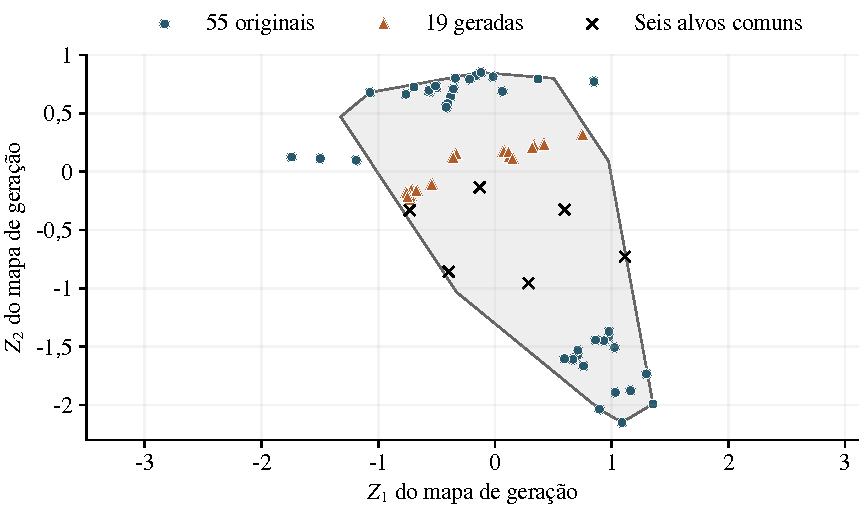
\includegraphics[width=\textwidth]{imgs/resultados/geracao_mapa_fixo.pdf}
\begin{singlespace}
{\small Legenda: círculos indicam as 55 originais; triângulos, as 19 adições;
cruzes, os seis alvos comuns às três sementes no primeiro lote de geração.
A região sombreada é o domínio interno. Os alvos adaptativos do segundo
lote não estão representados.\par}
{\fonte{elaboração própria a partir das coordenadas do experimento de geração.}}
\end{singlespace}
\end{figure}

A Tabela~\ref{tab:res-cobertura} compara as sequências e sua união sobre
o mesmo domínio e os mesmos 10.000 pontos Sobol. Na união, a distância
máxima diminuiu 20,92\%, a média diminuiu 36,27\% e a ocupação passou de
15\% para 20\%. Entretanto, 52,54\% dos pontos continuaram acima do limiar
de subcobertura, e a união não superou a melhor semente na distância
máxima. Houve preenchimento parcial, com lacunas remanescentes.

\begin{table}[!htbp]
\centering
\caption{Cobertura antes e depois das adições no mapa de geração fixo.}
\label{tab:res-cobertura}
\begin{singlespace}
\normalsize
\setlength{\tabcolsep}{5pt}
\renewcommand{\arraystretch}{1.15}
\begin{tabular}{lrrrrr}
\hline\hline
\textbf{Coleção} & \textbf{Adições} & \textbf{\shortstack{Distância\\máxima}} & \textbf{\shortstack{Distância\\média}} & \textbf{\shortstack{Subcobertura\\(\%)}} & \textbf{\shortstack{Ocupação\\(\%)}} \\
\hline
Base original & 0 & 1,2401 & 0,5284 & 71,70 & 15 \\
20260612 & 7 & 0,9875 & 0,3426 & 54,29 & 19 \\
104729 & 6 & 0,9853 & 0,3615 & 57,44 & 18 \\
1299709 & 6 & 0,9807 & 0,3640 & 59,86 & 18 \\
União das 19 & 19 & 0,9807 & 0,3368 & 52,54 & 20 \\
\hline\hline
\end{tabular}
\par\smallskip
{\small Nota: mesmas transformações, mesmo domínio interno e mesmos 10.000 pontos Sobol em todas as linhas. A ocupação usa uma grade $10\times10$. A linha da união foi recalculada com as coordenadas das 19 aceitações, sem repetir a geração.\par}
{\fonte{elaboração própria a partir dos dados experimentais.}}
\end{singlespace}
\end{table}


O resultado demonstra maior cobertura dessa representação, não de todo
o conjunto de instâncias possíveis do WSP. A ausência de geração aleatória
sob igual orçamento também impede estimar a vantagem da orientação por ISA.

\section{Desempenho dos métodos na coleção ampliada}\label{sec:res-benchmark}

\subsection{Resultados gerais e diferenças entre coleções}

A Tabela~\ref{tab:res-desempenho} resume as 656 execuções por método,
com peso igual por instância. O IBS, adotado como método de referência,
apresentou o menor \textit{gap} médio
global, 3,49\%, e a melhor média em 44 casos, incluindo 37 vitórias
exclusivas. MIP teve \textit{gap} de 15,06\%, mas posição média próxima
à do IBS: frequência das colocações e magnitude das perdas são aspectos
diferentes da comparação.

\begin{table}[!htbp]
\centering
\caption{Desempenho dos seis métodos por coleção.}
\label{tab:res-desempenho}
\begin{singlespace}
\normalsize
\setlength{\tabcolsep}{5pt}
\renewcommand{\arraystretch}{1.15}
\begin{tabular}{lrrrrrr}
\hline\hline
\textbf{Método} & \textbf{\shortstack{\textit{Gap} 55\\(\%)}} & \textbf{\shortstack{\textit{Gap} 19\\(\%)}} & \textbf{\shortstack{\textit{Gap} 74\\(\%)}} & \textbf{\shortstack{Posição\\média}} & \textbf{\shortstack{Melhor\\média}} & \textbf{\shortstack{Melhor média\\exclusiva}} \\
\hline
IBS & 2,65 & 5,92 & 3,49 & 2,07 & 44 & 37 \\
MIP & 18,52 & 5,04 & 15,06 & 2,16 & 11 & 6 \\
CUTH & 29,39 & 3,23 & 22,67 & 2,80 & 20 & 20 \\
LBBD & 38,11 & 9,67 & 30,81 & 4,39 & 11 & 4 \\
ILS & 39,57 & 10,03 & 31,98 & 5,32 & 1 & 0 \\
RS & 43,75 & 9,05 & 34,84 & 4,26 & 0 & 0 \\
\hline\hline
\end{tabular}
\par\smallskip
{\small Nota: \textit{gaps} médios com peso igual por instância. As duas falhas ILS permanecem na análise com a solução viável sem recursos. A coluna melhor média inclui empates; a última coluna conta somente vitórias exclusivas.\par}
{\fonte{elaboração própria a partir dos dados experimentais.}}
\end{singlespace}
\end{table}


O IBS liderou a base original com \textit{gap} médio de 2,65\%, em
consonância com o desempenho favorável relatado por
\citeonline{DelazeriRitt2024,DelazeriRitt2026}, embora os protocolos não
sejam idênticos. Nas adições, CUTH obteve a menor média, 3,23\%, e liderou
15 casos; IBS e MIP lideraram dois cada. A Figura~\ref{fig:res-ibs-cuth}
evidencia esse contraste. A ampliação revelou um regime favorável à CUTH
que a média da coleção original representava pouco.

\begin{figure}[!htbp]
\centering
\caption{Comparação dos \textit{gaps} médios do IBS e de CUTH por instância.}
\label{fig:res-ibs-cuth}
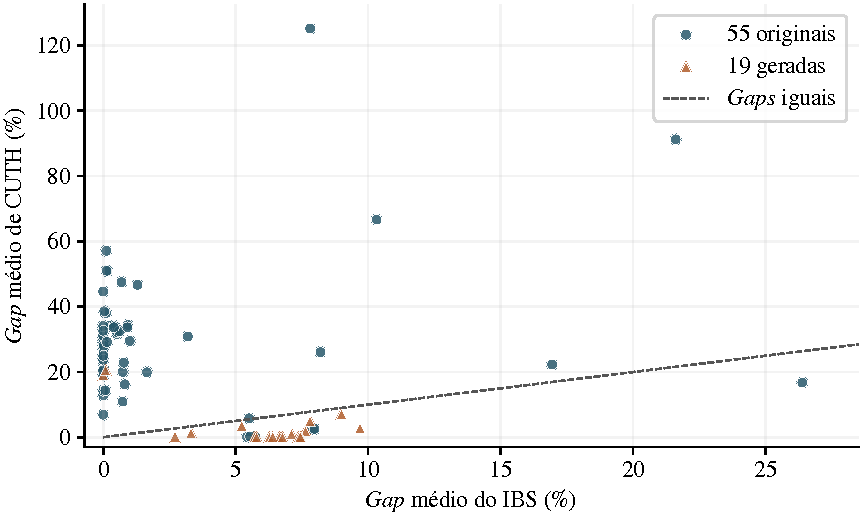
\includegraphics[width=\textwidth]{imgs/resultados/ibs_cuth_instancias.pdf}
\begin{singlespace}
{\small Legenda: cada ponto representa uma instância. Abaixo da igualdade,
CUTH tem menor \textit{gap}; acima, IBS.\par}
{\fonte{elaboração própria a partir dos objetivos reavaliados do experimento.}}
\end{singlespace}
\end{figure}

\subsection{Tamanho, origem e escala dos \textit{gaps}}

IBS apresentou o menor \textit{gap} médio em \textit{Small},
\textit{Medium} e \textit{Large}, e CUTH, em \textit{Huge}
(Tabela~\ref{tab:res-classes}). Essa última classe contém nove adições e
três originais: o \textit{gap} médio de CUTH foi aproximadamente 0,00249\%
nas primeiras e 9,50\% nas últimas. Portanto, o porte não explica sozinho
sua vantagem. Tampouco houve domínio uniforme nas adições: em
\textit{Large}-\texttt{027de052}, CUTH teve 19,03\%, enquanto IBS teve 0,00\%.
Nas adições, CUTH apresentou a menor média nas nove \textit{Huge},
em três das seis \textit{Large} e nas três \textit{Medium}; a única
\textit{Small} foi liderada por MIP. Assim, suas 15 lideranças se
distribuíram por três classes de tamanho.

\begin{table}[!htbp]
\centering
\caption{\textit{Gap} médio por classe de tamanho na coleção de 74 instâncias.}
\label{tab:res-classes}
\begin{singlespace}
\normalsize
\setlength{\tabcolsep}{5pt}
\renewcommand{\arraystretch}{1.15}
\begin{tabular}{lrrrr}
\hline\hline
\textbf{Método} & \textbf{\shortstack{\textit{Small}\\($n=20$)}} & \textbf{\shortstack{\textit{Medium}\\($n=33$)}} & \textbf{\shortstack{\textit{Large}\\($n=9$)}} & \textbf{\shortstack{\textit{Huge}\\($n=12$)}} \\
\hline
IBS & 0,73 & 3,43 & 5,38 & 6,81 \\
MIP & 3,47 & 25,81 & 11,79 & 7,27 \\
CUTH & 23,83 & 31,78 & 13,78 & 2,38 \\
LBBD & 8,01 & 54,73 & 22,46 & 9,31 \\
ILS & 9,49 & 56,18 & 23,29 & 9,42 \\
RS & 29,25 & 51,28 & 21,12 & 9,21 \\
\hline\hline
\end{tabular}
\par\smallskip
{\small Nota: valores em porcentagem, com peso igual por instância. Cada classe contém instâncias originais e geradas.\par}
{\fonte{elaboração própria a partir dos dados experimentais.}}
\end{singlespace}
\end{table}


A escala do BKV exige cautela. Nas nove \textit{Huge} geradas, a melhor
perda observada corresponde a 92,84\%--94,55\% dos 6.400 vértices.
A solução sem recursos já apresenta \textit{gap} médio de 6,80\% nesses
casos, apesar da queima total antes do horizonte. Na coleção original,
seu \textit{gap} médio é 51,12\%; nas adições, 10,10\%. Logo, percentuais
pequenos não demonstram perdas absolutas pequenas nem dificuldade
uniformemente baixa. A solução sem recursos serve aqui à interpretação
da escala e não integra o ranking como um sétimo método.

\subsection{Comparações pareadas}

Além da média global, comparou-se a frequência com que cada método
superou outro nas 74 instâncias. Em cada comparação, considerou-se vencedor
o método com menor \textit{gap} médio nas repetições daquela instância;
os empates foram registrados separadamente. Essa contagem distingue vencer
em muitas instâncias de obter uma grande vantagem em poucas delas.

Aplicou-se o teste de sinal para avaliar o desequilíbrio entre vitórias
e derrotas, excluindo os empates. Como os seis métodos formam 15 pares,
os valores de $p$ receberam a correção de Holm para controlar o risco de
identificar diferenças indevidamente ao realizar múltiplos testes.
Adotou-se o limiar de 0,05: resultados com $p$ ajustado menor ou igual
a esse valor foram considerados estatisticamente significativos.

O IBS apresentou menor média que CUTH em 51 instâncias, enquanto CUTH
venceu nas outras 23. O $p$ ajustado de aproximadamente 0,006065 ficou
abaixo do limiar adotado, indicando uma vantagem estatisticamente
significativa do IBS na frequência de vitórias. Contra MIP, o IBS venceu
42 vezes, empatou cinco e perdeu 27. Nesse caso, o $p$ ajustado de
0,182373 ficou acima de 0,05: o placar favoreceu IBS, mas a evidência foi
insuficiente para concluir uma diferença estatisticamente significativa.
Esse resultado também não demonstra equivalência entre os dois métodos.

A frequência de vitórias deve ser interpretada junto da magnitude dos
\textit{gaps}. A RS, utilizada como linha de base, superou ILS em 58
instâncias e perdeu em 16; contra
LBBD, venceu em 50 e perdeu em 24. Ainda assim, seu \textit{gap} médio
global foi maior que o de ambos. Isso ocorre porque a contagem atribui
uma vitória tanto a uma diferença pequena quanto a uma grande, enquanto
a média global incorpora o tamanho das diferenças. Assim, vencer mais
vezes não garante menor \textit{gap} médio na coleção.

Esses testes têm caráter exploratório. As instâncias foram reunidas por
seleção dirigida, e algumas compartilham o mesmo grafo de propagação.
Por isso, não constituem uma amostra aleatória de problemas independentes.
A correção de Holm considera as múltiplas comparações, mas não elimina
essas limitações; as conclusões estatísticas devem ser interpretadas no
contexto da coleção e do protocolo utilizados.

\subsection{Tratamento de falhas e tempos de execução}

A interpretação do desempenho também depende do tratamento das falhas e
das soluções retornadas ao final do tempo disponível. Nas duas execuções
em que ILS falhou, utilizou-se, para pontuação, a solução viável que não
aplica recursos. As falhas foram, portanto, mantidas no cálculo das médias.
Excluí-las reduziria o \textit{gap} global de ILS de 31,9818\% para
31,9770\%, sem alterar sua posição na comparação entre métodos.

Os valores utilizados nas tabelas foram calculados a partir da avaliação
das soluções salvas. Em uma execução de MIP, por exemplo, o registro
indicava 295 vértices queimados, mas a reavaliação da solução pelo modelo
adotado resultou em 283. Esse último valor foi utilizado nos resumos,
preservando-se o registro original. O caso reforça a necessidade de
aplicar a mesma regra de avaliação às soluções dos diferentes métodos.

Na implementação de LBBD, a inicialização heurística e a etapa exata
compartilharam o mesmo limite de tempo. A etapa exata chegou a ser
iniciada em 193 das 656 execuções, o que não significa que tenha sido
concluída nesses casos. Em 274 execuções, o procedimento retornou a
solução sem recursos por não dispor de uma solução viável utilizável
ao término da execução. Portanto, o desempenho observado corresponde
ao procedimento completo sob o orçamento de tempo adotado, incluindo
a inicialização e a alternativa prevista para ausência de solução.

Quanto ao tempo total de execução, CUTH apresentou mediana de 1,01
segundo, enquanto IBS, MIP e RS tiveram medianas próximas de 1.350
segundos. Esses valores agregam execuções de diferentes classes de
tamanho e não informam quanto tempo cada método levaria para alcançar
uma mesma qualidade de solução. Na base original, por exemplo, a menor
duração das execuções de CUTH acompanhou \textit{gaps} mais altos.
Assim, tempo e qualidade precisam ser considerados conjuntamente na
interpretação dos resultados.

\section{Representações ISA e contribuição da topologia}\label{sec:res-isa}

\subsection{Seleção de atributos e organização dos mapas}

A ISA considerou quatro famílias de instâncias, definidas pela coleção
(55 ou 74 instâncias) e pelos atributos candidatos: controle, com 35
atributos originais; ou topologia, com 107 candidatos que incluem medidas
topológicas adicionais. Cada família foi analisada por um modelo próprio,
denominado 55-controle, 55-topologia, 74-controle ou 74-topologia.
Todos usaram os desempenhos do mesmo experimento comparativo, com seis
colunas de algoritmos. Nos modelos de 55 instâncias, utilizaram-se apenas
as linhas correspondentes às originais da matriz de 74 instâncias.
Cada modelo selecionou dez atributos (Tabela~\ref{tab:res-atributos-isa}).

\begin{table}[!htbp]
\centering
\caption{Atributos selecionados nos quatro modelos de ISA.}
\label{tab:res-atributos-isa}
\begin{singlespace}
\small
\setlength{\tabcolsep}{3pt}
\renewcommand{\arraystretch}{1.02}
\begin{tabular}{>{\raggedright\arraybackslash}p{0.46\textwidth}ccccr}
\hline\hline
\noalign{\vskip 4pt}
\textbf{Atributo} & \textbf{\shortstack{55\\controle}} & \textbf{\shortstack{55\\topologia}} & \textbf{\shortstack{74\\controle}} & \textbf{\shortstack{74\\topologia}} & \textbf{\shortstack{Nº de\\modelos}} \\
\hline
\multicolumn{6}{l}{\textbf{Originais}} \\
\multicolumn{6}{l}{\textit{Recursos e atraso}} \\
Recursos totais & $\times$ & $\times$ &  & $\times$ & 3 \\
Número de liberações de recursos & $\times$ &  & $\times$ &  & 2 \\
Recursos por liberação &  &  & $\times$ &  & 1 \\
Atraso/$H$ & $\times$ &  & $\times$ &  & 2 \\
\multicolumn{6}{l}{\textit{Liberações}} \\
Primeira liberação/$H$ & $\times$ &  & $\times$ &  & 2 \\
Última liberação/$H$ &  &  & $\times$ &  & 1 \\
Janela de liberação/$H$ & $\times$ & $\times$ &  &  & 2 \\
\multicolumn{6}{l}{\textit{Tempos dos arcos}} \\
Média dos tempos dos arcos &  &  &  & $\times$ & 1 \\
Desvio padrão dos tempos dos arcos & $\times$ &  &  &  & 1 \\
Primeiro quartil dos tempos dos arcos & $\times$ &  &  &  & 1 \\
Mediana dos tempos dos arcos &  &  & $\times$ &  & 1 \\
Terceiro quartil dos tempos dos arcos &  & $\times$ &  &  & 1 \\
CV dos tempos dos arcos &  &  &  & $\times$ & 1 \\
\multicolumn{6}{l}{\textit{Assimetria e coordenadas}} \\
Assimetria direcional média & $\times$ & $\times$ & $\times$ &  & 3 \\
Amplitude das coordenadas $x$ &  &  &  & $\times$ & 1 \\
Amplitude das coordenadas $y$ &  &  & $\times$ &  & 1 \\
\multicolumn{6}{l}{\textit{Chegadas sem recursos}} \\
Maior chegada sem recursos/$H$ &  &  & $\times$ &  & 1 \\
Percentil 5 das chegadas/$H$ &  &  &  & $\times$ & 1 \\
Mediana das chegadas/$H$ & $\times$ &  &  &  & 1 \\
Percentil 95 das chegadas/$H$ &  & $\times$ &  &  & 1 \\
\multicolumn{6}{l}{\textit{Chegadas entre liberações}} \\
Média de chegadas entre liberações & $\times$ & $\times$ &  & $\times$ & 3 \\
Máximo de chegadas entre liberações &  &  & $\times$ &  & 1 \\
\multicolumn{6}{l}{\textbf{Topológicos}} \\
\multicolumn{6}{l}{\textit{Centralidade harmônica}} \\
Harmônica de saída (distância): média &  & $\times$ &  &  & 1 \\
Harmônica de entrada (distância): média &  &  &  & $\times$ & 1 \\
\multicolumn{6}{l}{\textit{HITS}} \\
Autoridade HITS (força): mediana &  & $\times$ &  &  & 1 \\
Autoridade HITS (força): terceiro quartil &  &  &  & $\times$ & 1 \\
Autoridade HITS (força): desvio padrão &  &  &  & $\times$ & 1 \\
\textit{Hub} HITS (força): desvio padrão &  & $\times$ &  &  & 1 \\
\multicolumn{6}{l}{\textit{PageRank}} \\
PageRank ponderado: média &  & $\times$ &  &  & 1 \\
PageRank ponderado: mínimo &  &  &  & $\times$ & 1 \\
\hline
\textbf{Total selecionado} & 10 & 10 & 10 & 10 & \\
\hline\hline
\end{tabular}
\par\smallskip
{\small Nota: $\times$ indica seleção; célula vazia, ausência. Nº de modelos indica em quantos dos quatro modelos o atributo foi selecionado. Grupos originais seguem a Tabela~\ref{tab:met-atributos-originais}, reunindo assimetria e coordenadas. Harmônica designa a centralidade harmônica; distância usa os tempos dos arcos e força, seus inversos. Chegadas são calculadas sem recursos.\par}
{\fonte{elaboração própria a partir das seleções dos modelos finais.}}
\end{singlespace}
\end{table}


Os quatro modelos selecionaram, ao todo, 30 atributos distintos.
Nenhum aparece nos quatro modelos. Apenas recursos totais, assimetria
direcional média e média de chegadas entre liberações aparecem em três;
quatro atributos aparecem em dois e os outros 23, em apenas um.
A recorrência é maior quando se consideram as famílias de atributos:
todos os modelos selecionam ao menos um descritor de recursos e atraso,
um de tempos dos arcos e um de chegadas sem recursos. Nos tempos dos
arcos, por exemplo, alternam-se média, desvio padrão, quartis, mediana
e coeficiente de variação.

Nos modelos 55-topologia e 74-topologia, quatro dos dez atributos
selecionados são topológicos, mas nenhum desses quatro se repete de
um modelo para o outro. Ainda assim, ambos selecionam descritores das
famílias de centralidade harmônica, autoridade HITS e PageRank, com
direções ou estatísticas diferentes. Portanto, a semelhança entre os
modelos aparece mais nas famílias representadas do que na identidade
dos atributos escolhidos.

A seleção do SIFTED minimiza o erro interno de classificação do
desempenho. A alternância entre resumos de uma mesma família é
compatível com a presença de candidatos que descrevem propriedades
relacionadas, como média, mediana e quartis dos tempos dos arcos.
Como foi usada uma única semente por modelo, essas diferenças descrevem
as quatro configurações obtidas; não medem a estabilidade da seleção
sob novas sementes, conforme a Seção~\ref{sec:met-limitacoes}.

Parte dos atributos topológicos também expressa tamanho. No modelo
55-topologia, essa relação é explícita:
como os escores de PageRank somam um, sua média equivale a $1/|V|$.
No modelo 74-topologia, uma verificação descritiva também identificou
forte associação com o tamanho. O terceiro quartil da autoridade HITS
e o mínimo do PageRank apresentaram correlações de Spearman com $|V|$
de $-0{,}9206$ e $-0{,}9600$, respectivamente. Os mesmos coeficientes
foram obtidos para $|A|$, pois, nesta coleção, as quantidades de vértices
e arcos têm exatamente a mesma ordenação, incluindo os empates.
A normalização de PageRank e HITS para soma um
(Seção~\ref{sec:met-topologia}) ajuda a interpretar os sinais negativos:
ao distribuir a mesma soma entre mais vértices, a média dos escores
diminui para $1/|V|$. Esse efeito de escala pode contribuir para os
menores valores dos resumos nodais observados nos grafos maiores.

A Figura~\ref{fig:res-isa} apresenta os quatro mapas. Como cada modelo
tem transformações, escala e orientação próprias, a comparação considera
a organização relativa das instâncias, em vez de confrontar diretamente
suas coordenadas. No modelo 74-controle, as novas instâncias se concentram acima do agrupamento
principal de originais, enquanto outro grupo de originais ocupa a região
inferior direita. No modelo 74-topologia, as novas instâncias se distribuem pela região inferior
esquerda e pela região central, com algumas próximas de originais.
Portanto, a separação visual entre originais e adições depende também
do conjunto de atributos e do modelo ajustado.

Para comparar a organização dos mapas, calculou-se a correlação de
Spearman entre as distâncias dos mesmos pares de instâncias. Esse
coeficiente varia de $-1$ a $1$; valores próximos de $1$ indicam que
a ordenação dos pares, dos mais próximos aos mais distantes, é
semelhante nos dois mapas. Nas 74 instâncias, os modelos 74-controle e
74-topologia não compartilham atributos selecionados, mas apresentam
correlação de 0,8484 entre as distâncias. Suas predições coincidem em
420 das 444 classificações de bom ou não bom desempenho, uma para cada
combinação de instância e algoritmo ($74\times6$), totalizando 94,59\%.

Entre os modelos 55-topologia e 74-topologia, os dois atributos mantidos
são recursos totais e média de chegadas entre liberações. A comparação
restrita às 55 instâncias comuns apresenta correlação de 0,9540 entre
as distâncias e concordância em 327 das 330 classificações ($55\times6$),
ou 99,09\%. Conjuntos distintos de atributos podem, portanto, produzir
organizações semelhantes das mesmas instâncias.

O alinhamento de Procrustes complementa essa comparação ao retirar
diferenças globais de posição, orientação e escala dos mapas. Nas 55
instâncias comuns, o deslocamento médio após a ampliação foi 0,0487 no
controle e 0,0215 com topologia, indicando menor alteração geométrica
nesse segundo modelo. Nos contrastes entre controle e topologia, os
deslocamentos médios foram 0,0409 para as 55 instâncias e 0,0551 para
as 74. Esses valores usam coordenadas normalizadas: descrevem mudanças
na representação, sem medir distância física ou acerto das classificações.

A concordância mede a coincidência entre as respostas dos modelos,
e não o acerto em relação aos rótulos observados. Sua interpretação
também depende do desbalanceamento das classes, que pode favorecer
respostas coincidentes. No IBS, por exemplo, 70 das 74 instâncias
recebem o rótulo bom, conforme discutido na
Seção~\ref{sec:res-isa-diagnosticos}.

A topologia participa da seleção com quatro dos dez atributos nos
dois modelos que a incluem, mas os descritores mudam entre as coleções
e parte deles acompanha o tamanho dos grafos. A
Seção~\ref{sec:res-isa-diagnosticos} examina se sua inclusão também
se traduz em ganhos no diagnóstico preditivo.

\begin{figure}[!htbp]
\centering
\caption{Representações PILOT dos quatro modelos finais de ISA.}
\label{fig:res-isa}
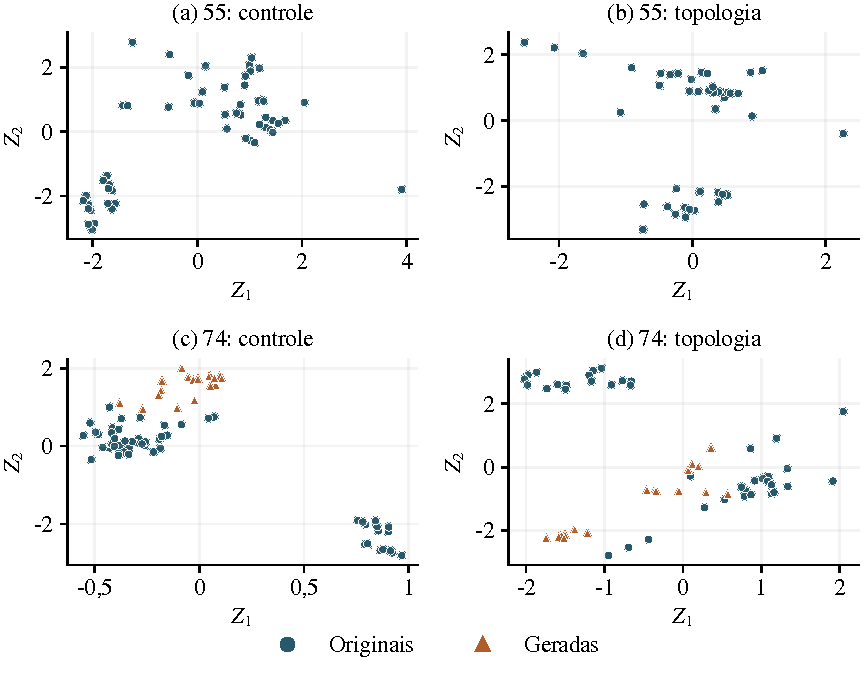
\includegraphics[width=\textwidth]{imgs/resultados/isa_quatro_modelos.pdf}
\begin{singlespace}
{\small Legenda: círculos indicam originais; triângulos, adições.
Escalas e orientações pertencem a cada ajuste; distâncias entre mapas
não são diretamente comparáveis.\par}
{\fonte{elaboração própria a partir das coordenadas dos modelos finais.}}
\end{singlespace}
\end{figure}

\FloatBarrier
\subsection{Diagnósticos internos e desbalanceamento dos rótulos}
\label{sec:res-isa-diagnosticos}

O rótulo bom, definido por \textit{gap} de até 10\%, não identifica o líder.
O IBS o recebeu em 70 das 74 instâncias, inclusive nas 19 adições, embora
liderasse somente duas delas. A solução sem recursos já satisfaz esse
limiar em 14 adições, incluindo as nove \textit{Huge}; assim, nem todas
ampliaram a dificuldade da classificação. Nos dois modelos de 74,
PYTHIA classificou todos os casos como bons para IBS: a acurácia simples
foi 94,59\%, mas a acurácia balanceada foi 50\%, pois nenhum dos quatro
negativos foi reconhecido.

A Tabela~\ref{tab:res-cv} apresenta o diagnóstico auxiliar repetido.
Nas 74 instâncias, a topologia elevou a média em 5,74 pontos percentuais
para ILS, 4,04 para LBBD e 5,12 para RS. CUTH e MIP perderam aproximadamente
0,73 e 0,31 ponto, e IBS permaneceu em 50,71\%. Os resultados nas 55
também variam entre métodos. Portanto, há contribuição descritiva e ganhos
internos específicos, sem melhora uniforme.

\begin{table}[!htbp]
\centering
\caption{Acurácia balanceada no diagnóstico auxiliar repetido.}
\label{tab:res-cv}
\begin{singlespace}
\normalsize
\setlength{\tabcolsep}{5pt}
\renewcommand{\arraystretch}{1.15}
\begin{tabular}{lrrrr}
\hline\hline
\textbf{Método} & \textbf{\shortstack{55\\controle}} & \textbf{\shortstack{55\\topologia}} & \textbf{\shortstack{74\\controle}} & \textbf{\shortstack{74\\topologia}} \\
\hline
IBS & $53{,}33\pm1{,}15$ & $53{,}33\pm1{,}15$ & $50{,}71\pm0{,}00$ & $50{,}71\pm0{,}00$ \\
MIP & $88{,}37\pm2{,}24$ & $89{,}80\pm2{,}58$ & $90{,}21\pm1{,}40$ & $89{,}90\pm2{,}67$ \\
CUTH & $84{,}69\pm6{,}29$ & $81{,}06\pm4{,}45$ & $91{,}72\pm1{,}15$ & $90{,}99\pm2{,}59$ \\
LBBD & $91{,}90\pm2{,}01$ & $93{,}14\pm1{,}81$ & $91{,}56\pm2{,}61$ & $95{,}60\pm0{,}92$ \\
ILS & $94{,}33\pm2{,}18$ & $94{,}55\pm1{,}33$ & $89{,}33\pm2{,}25$ & $95{,}07\pm1{,}09$ \\
RS & $91{,}94\pm8{,}08$ & $88{,}40\pm1{,}58$ & $87{,}92\pm1{,}64$ & $93{,}03\pm2{,}24$ \\
\hline\hline
\end{tabular}
\par\smallskip
{\small Nota: média em porcentagem $\pm$ desvio padrão amostral em pontos percentuais, em dez repetições de quatro partições. Coordenadas e hiperparâmetros foram obtidos globalmente; o procedimento não é aninhado nem externo.\par}
{\fonte{elaboração própria a partir dos dados experimentais.}}
\end{singlespace}
\end{table}


Como coordenadas e hiperparâmetros foram obtidos globalmente, esses valores
não estimam generalização externa do fluxo completo. O desvio padrão
resume dez repetições do particionamento; a seleção de atributos do SIFTED
usou uma única semente por ajuste, cuja estabilidade não é medida por essas
repetições. A leitura deve considerar
a diversidade da base, não apenas altas taxas de acerto, conforme a
perspectiva da ISA \cite{SmithMilesMunoz2023}.

Os \textit{footprints} mostram como essas predições se traduzem em regiões
de bom desempenho (Tabela~\ref{tab:res-footprints}). Nos quatro modelos,
o \textit{footprint} do IBS ocupa 100\% da área de referência construída pelo TRACE,
com densidade relativa e pureza iguais a um. Essa pureza é calculada a
partir das classes previstas, e não dos rótulos observados. Assim, a região
extensa acompanha a classificação generalizada como bom, mas não identifica
os casos em que o IBS ultrapassa o limiar de \textit{gap}. Para os demais
métodos, as regiões ocupam frações menores ou não chegam a ser construídas.
As diferenças entre mapas descrevem as respectivas geometrias e predições;
uma área maior não demonstra, por si só, maior competência observada.

\begin{table}[!htbp]
\centering
\caption{Área relativa dos footprints de bom desempenho nos quatro modelos.}
\label{tab:res-footprints}
\begin{singlespace}
\normalsize
\setlength{\tabcolsep}{7pt}
\renewcommand{\arraystretch}{1.12}
\begin{tabular}{lrrrr}
\hline\hline
\noalign{\vskip 3pt}
\textbf{Método} & \textbf{\shortstack{55\\controle}} & \textbf{\shortstack{55\\topologia}} & \textbf{\shortstack{74\\controle}} & \textbf{\shortstack{74\\topologia}} \\
\hline
IBS & 100,00 & 100,00 & 100,00 & 100,00 \\
MIP & 15,64 & 39,82 & 54,47 & 26,33 \\
CUTH & 0,00 & 0,00 & 4,38 & 11,07 \\
LBBD & 15,64 & 39,82 & 38,78 & 28,93 \\
ILS & 15,64 & 39,82 & 38,78 & 28,93 \\
RS & 0,00 & 0,00 & 4,38 & 6,47 \\
\hline\hline
\end{tabular}
\par\smallskip
{\small Nota: área do footprint dividida pela área de referência construída pelo TRACE no próprio mapa, em porcentagem. As regiões usam classes previstas, não rótulos observados. Zero indica ausência de região construída, não prova de incapacidade do método. As áreas absolutas de mapas diferentes não são diretamente comparáveis.\par}
{\fonte{elaboração própria a partir dos resultados dos quatro modelos.}}
\end{singlespace}
\end{table}


\section{Trajetórias de busca do IBS}\label{sec:res-stns}

\subsection{Instâncias clássicas no protocolo histórico}

As 160 execuções clássicas produziram 16 redes filtradas, com 10 a 37 nós.
LA0 apresentou 13 nós e fração compartilhada de 0,769, enquanto LB4 teve
31 nós, fração de 0,032 e oito assinaturas finais fora do conjunto de
melhor avaliação (Figura~\ref{fig:res-stn-classicas}). Esses casos contrastam
reutilização e dispersão das assinaturas. Suas forças de entrada limitadas,
0,6 e 0,1, descrevem frequências normalizadas, não probabilidades de sucesso.

O cruzamento das 16 redes com a PCA exploratória e os rótulos históricos
incluiu dez instâncias rotuladas como IBS, três como MIP e três como
LBBD ou ILS. As faixas de coordenadas desses grupos se sobrepunham nos
dois eixos da PCA. A fração compartilhada média foi 13,08\% no grupo IBS,
38,90\% no grupo MIP e 35,64\% nos demais; a média de estados finais não
melhores variou de 4,9 a 6,0 entre os grupos. Portanto, casos próximos
nessa representação podiam apresentar recorrências diferentes, e o rótulo
de melhor método não correspondia a um único perfil de trajetória do IBS.
Os dois grupos com três casos limitam a interpretação; esses rótulos
pertencem à exploração histórica, não à comparação final das 74 instâncias.

\begin{figure}[!htbp]
\centering
\caption{STNs históricas filtradas das instâncias LA0 e LB4.}
\label{fig:res-stn-classicas}
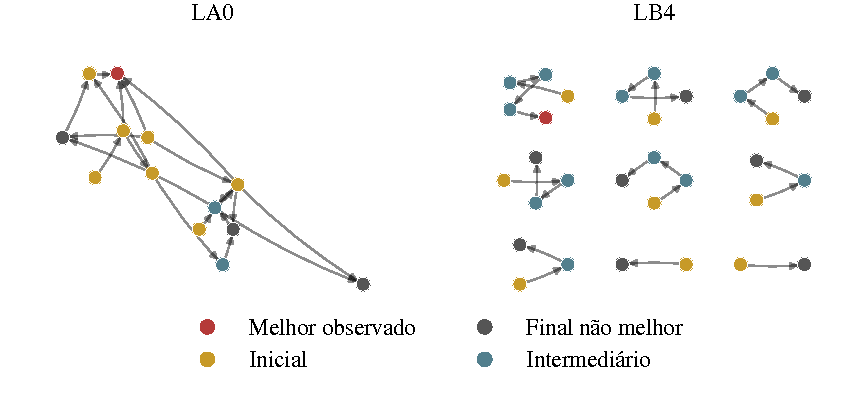
\includegraphics[width=\textwidth]{imgs/resultados/stns_classicas.pdf}
\begin{singlespace}
{\small Legenda: nós representam conjuntos protegidos e arestas conectam
assinaturas consecutivas na sequência filtrada. Melhor indica o menor
objetivo observado na rede; posições são apenas um arranjo gráfico.\par}
{\fonte{elaboração própria a partir dos registros históricos filtrados.}}
\end{singlespace}
\end{figure}

As redes complementam o objetivo final ao descrever o percurso
\cite{OchoaMalanBlum2021}. Entretanto, assinaturas sem instantes, orçamento
menor e limite de iterações impedem atribuir diferenças entre redes
históricas e adicionais isoladamente à expansão da coleção.

\subsection{Trajetórias suplementares com tempos decimais}

As 190 buscas adicionais, com tempos decimais preservados, produziram
36.593 registros e 2.682 estados distintos, contados por instância.
Houve 13.462 transições de piora, e todas as execuções apresentaram ao
menos uma. A última linha terminou pior que a incumbente em 123 buscas:
o desempenho final deve ser lido pela melhor solução preservada, não
pelo último estado da trajetória.

O filtro de não piora conservou 14.942 registros e 744 nós, mas pode ligar
assinaturas que não eram consecutivas no registro bruto. A rede filtrada
é uma sequência derivada; a bruta conserva os retornos a soluções piores.

O contraste por porte mostrou perfis diferentes nas redes brutas.
A única \textit{Small} apresentou 51 nós e Jaccard médio de 0,9412;
as três \textit{Medium}, de três a seis nós e Jaccard 1. Nas seis
\textit{Large}, os valores variaram de dois a 106 nós e Jaccard de
0,4500 a 1; nas nove \textit{Huge}, de 184 a 365 nós e Jaccard de
aproximadamente 0,0004 a 0,0774. Assim, as maiores redes das
\textit{Huge} acompanharam menor compartilhamento de estados entre
execuções. Como os limites de tempo também crescem com o porte, esse
contraste não isola o efeito do tamanho.

A Figura~\ref{fig:res-stn-suplementares} mostra
\textit{Large}-\texttt{00d0559e}, com dois estados e Jaccard 1, e
\textit{Huge}-\texttt{07952568}, com 365 estados e Jaccard 0,0173.
O primeiro caso atingiu objetivo 1.556 frente a BKV 1.515; o segundo,
6.355 frente a 5.942. Compartilhamento e diversidade não asseguram,
isoladamente, boa qualidade relativa.

\begin{figure}[!htbp]
\centering
\caption{Contraste entre duas STNs suplementares brutas do IBS.}
\label{fig:res-stn-suplementares}
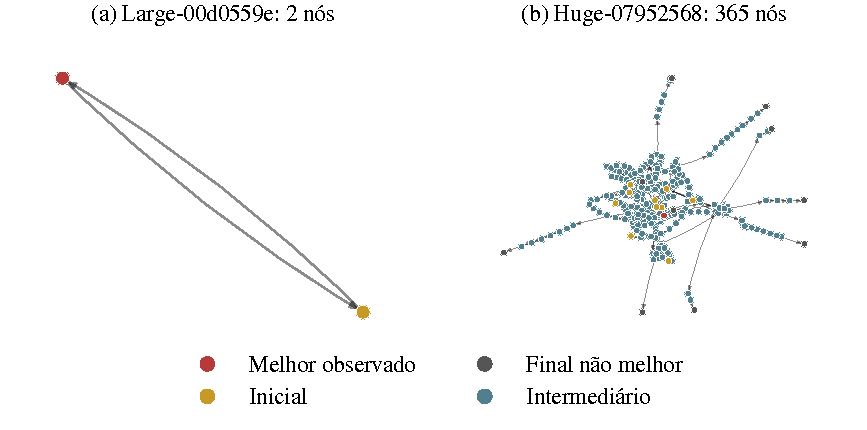
\includegraphics[width=\textwidth]{imgs/resultados/stns_suplementares.pdf}
\begin{singlespace}
{\small Legenda: dez execuções por instância. Nós são assinaturas
vértice--instante; arestas ligam estados consecutivos distintos.
As distâncias no desenho não representam diferenças de qualidade.\par}
{\fonte{elaboração própria a partir das redes brutas reconstruídas.}}
\end{singlespace}
\end{figure}

O tempo de parede excedeu o limite nominal nas 190 buscas, com excesso
relativo máximo de 5,28\%, pois o prazo é verificado entre chamadas
completas da busca em feixe. Ambiente e duração efetiva também diferiram
do histórico com tempos truncados, de modo que esse contraste não isola
o efeito da correção numérica. Nas \textit{Huge}, as STNs usam dez sementes,
enquanto as médias comparativas usam três.

\section{Relação entre instâncias, desempenho e trajetórias}\label{sec:res-integracao}

O cruzamento por identificador associou os descritores das STNs brutas
ao \textit{gap} médio IBS nas 19 adições (Tabela~\ref{tab:res-correlacoes}).
Nenhuma das cinco associações apresentou $p$ nominal inferior a 0,05.
Os descritores examinados não substituem diretamente a qualidade relativa,
sem que isso demonstre ausência de relações sob outros protocolos.
A interpretação considera a amostra dirigida e a diferença entre as
execuções usadas nas redes e no desempenho.

\begin{table}[!htbp]
\centering
\caption{Associação entre descritores das STNs brutas e \textit{gap} médio do IBS.}
\label{tab:res-correlacoes}
\begin{singlespace}
\normalsize
\setlength{\tabcolsep}{5pt}
\renewcommand{\arraystretch}{1.15}
\begin{tabular}{lrr}
\hline\hline
\textbf{Descritor} & \textbf{$\rho$ de Spearman} & \textbf{$p$ nominal} \\
\hline
Número de nós & 0,052 & 0,833 \\
Número de arestas & -0,133 & 0,586 \\
Finais distintos não melhores & 0,031 & 0,898 \\
Força de entrada sem teto & 0,328 & 0,171 \\
Jaccard médio & 0,004 & 0,989 \\
\hline\hline
\end{tabular}
\par\smallskip
{\small Nota: 19 instâncias geradas. Descritores das execuções complementares e \textit{gaps} do experimento comparativo, associados por instância. Correlações exploratórias, sem ajuste de multiplicidade nem interpretação causal.\par}
{\fonte{elaboração própria a partir dos dados experimentais.}}
\end{singlespace}
\end{table}


Em relação à hipótese da Seção~\ref{sec:pergunta-pesquisa}, a ampliação
revelou um regime favorável à CUTH, e as STNs distinguiram percursos não
descritos pelas médias finais. Na ISA, atributos topológicos foram
selecionados e sua inclusão alterou moderadamente a geometria dos mapas,
que mantiveram forte semelhança com o controle. A troca dos descritores
entre as coleções, sua associação parcial com o tamanho e os ganhos
preditivos heterogêneos não permitem concluir que a topologia ofereceu
informação independente dos atributos originais. Essa sustentação da
hipótese é descritiva: a mudança conjunta de porte, recursos e tempos
impede atribuir os contrastes exclusivamente à cobertura ou à topologia.
O estudo caracteriza a coleção avaliada, sem demonstrar causalidade,
generalização preditiva externa ou validade operacional em incêndios reais.

\chapter{\MakeUppercase{Conclusão}}\label{sec:conclusao}

Este trabalho caracterizou e ampliou a cobertura de uma representação do
espaço de instâncias do WSP, relacionando propriedades dos casos de teste,
desempenho de seis métodos e trajetórias do IBS. O estudo consolidou e
caracterizou uma base de 55 instâncias por atributos do problema e medidas
topológicas. A geração e a validação de 19 adições para regiões internas
pouco ocupadas do mapa fixo ampliaram a coleção para 74 instâncias.
Compararam-se seis abordagens e analisaram-se quatro famílias de instâncias
nas configurações de ISA. As trajetórias do IBS foram caracterizadas por
redes de soluções visitadas e transições entre elas. Essas contribuições
atendem aos objetivos da Seção~\ref{sec:objetivos}, preservando a distinção
entre o mapa fixo utilizado na geração, os modelos finais de desempenho
e os diferentes protocolos de registro da busca.

A geração orientada demonstrou a viabilidade de produzir instâncias
válidas para regiões internas pouco ocupadas do mapa de referência.
Das 36 buscas, que consumiram 72.000 avaliações, resultaram 19 instâncias
aceitas e distintas. Na união das adições, a maior distância dos pontos
amostrados à coleção diminuiu 20,92\%, e a distância média, 36,27\%.
A ocupação da grade passou de 15\% para 20\%. O preenchimento foi parcial:
52,54\% dos pontos amostrados ainda permaneceram acima do limiar de
subcobertura. Esses resultados respondem ao objetivo de ampliar a cobertura
da representação adotada, mas não demonstram cobertura do conjunto de
instâncias possíveis do WSP nem superioridade sobre uma geração aleatória
com orçamento equivalente.

As 3.936 execuções comparativas mostraram que a ampliação da coleção
revelou regimes de desempenho distintos. O IBS manteve o menor
\textit{gap} médio global, de 3,49\%, e a melhor média, incluindo empates,
em 44 das 74 instâncias. Nas 19 adições, a CUTH apresentou
\textit{gap} médio de 3,23\% e liderou 15 casos. Assim, a liderança global
de um método não substitui a análise dos grupos de instâncias em que
outros são competitivos. Como as adições também alteraram tamanho,
recursos, liberações e tempos de propagação, o estudo não identifica
qual dessas propriedades explica isoladamente a mudança de regime.
Além disso, um \textit{gap} pequeno pode coexistir com perda absoluta
elevada, como ocorreu nas instâncias \textit{Huge} geradas.

Nas duas famílias de instâncias com medidas topológicas adicionais,
quatro dos dez atributos selecionados foram topológicos. Os descritores
escolhidos não coincidiram entre as coleções, e parte deles acompanhou o
tamanho dos grafos. Sua inclusão alterou moderadamente a geometria dos
mapas, que permaneceram semelhantes aos de controle. Nas 74 instâncias,
o diagnóstico auxiliar melhorou
para ILS, LBBD e RS, enquanto CUTH e MIP apresentaram reduções e IBS
permaneceu no mesmo patamar. Na própria amostra, os classificadores do IBS
previram bom desempenho para todos os casos e tiveram acurácia balanceada
de 50\%, apesar da alta acurácia simples. A conclusão sobre topologia é,
portanto, descritiva e condicionada ao método e à configuração utilizada;
a generalização do fluxo completo não foi demonstrada.

As STNs acrescentaram uma perspectiva sobre o percurso da busca que o
objetivo final não fornece. As 160 execuções clássicas e as 190 execuções
nas adições evidenciaram diferenças de recorrência, compartilhamento e
dispersão. Os registros brutos também mostraram retornos a soluções piores
que a incumbente, reforçando a necessidade de distinguir a solução
representativa de cada iteração da melhor solução acumulada. Contudo,
número de nós, compartilhamento e força de entrada não funcionaram como
substitutos diretos da qualidade: nas 19 adições, não se identificou uma
associação monotônica sustentada entre os cinco descritores examinados
e o \textit{gap} médio do IBS. As diferenças de assinatura, parâmetros,
parada e duração efetiva impedem interpretar o contraste entre redes
históricas e adicionais como efeito isolado da expansão.

Em resposta à pergunta da Seção~\ref{sec:pergunta-pesquisa}, foi possível
relacionar perfis estruturais e temporais a grupos de desempenho e
caracterizar comportamentos de busca distintos na coleção ampliada.
A hipótese recebeu sustentação descritiva na identificação do regime
favorável à CUTH nas adições e na caracterização de percursos distintos
de busca. Para a topologia, o resultado se restringe à seleção de
descritores e às alterações moderadas na geometria, com ganhos preditivos
heterogêneos, sem demonstrar informação independente do tamanho.
Não se demonstrou que o aumento de cobertura tenha causado as diferenças
observadas, nem que toda relação detectada dependa da ampliação.

As limitações da Seção~\ref{sec:met-limitacoes} delimitam essas conclusões
à coleção dirigida e aos protocolos avaliados.

Como trabalhos futuros, recomenda-se avaliar o fluxo ISA em instâncias
externas ou por validação aninhada, repetindo o fluxo completo dentro de
cada partição de treinamento e considerando o compartilhamento de
grafos na separação dos dados. Também são prioritárias a sensibilidade
a outros limiares de \textit{gap}, a comparação da geração orientada com
uma geração aleatória sob igual orçamento e a avaliação conjunta da perda
absoluta e do ganho em relação à solução sem recursos. Experimentos que
variem propriedades de forma controlada podem investigar os regimes
favoráveis à CUTH. Para as trajetórias, um protocolo comum de assinatura,
parada e amostragem permitiria comparações mais diretas entre coleções e,
posteriormente, entre métodos.

O contraste central foi a liderança de CUTH em 15 das 19 adições,
incluindo as nove \textit{Huge} e três das seis \textit{Large}, apesar
do menor \textit{gap} médio global do IBS. A média da coleção completa
não evidencia, sozinha, esse regime favorável à CUTH. A ampliação da
base mostrou, assim, que a avaliação dos métodos depende dos perfis
representados e deve considerar seus resultados por grupo, além da
classificação global.
O alcance do estudo é computacional e experimental, sem validar cenários
reais de incêndio nem prescrever decisões operacionais.


%==============================================================================
% Bibliografia

% Carrega o estilo para referências ABNT
\bibliographystyle{abntex2-alf}            

% Alterando informações do estilo de citação.
% Como estamos usando uma versão alterada, essas opções são necessárias.
% Et al. em itálico
\citeoption{abnt-etal-text=it}

% Até 3 autores antes do et al.
\citeoption{abnt-etal-cite=3}

% Colocar s.d. na falta de um ano de publicação
\citeoption{abnt-missing-year=sd}

% Altera o estilo de citação para (Autor, ano)
% A opção abnt-cite-style=AuthorYEAR está quebrada; essa é equivalente.
\citeoption{abnt-nbr10520=1988}
\citeoption{abnt-and-type=e}


% Comando necessário para corrigir o título das referências.
% Para o estilo ABNT, esse comando SEMPRE deve ser
% chamado antes do \bibliography
\referencias
% Adiciona as referência em bibtex 
\bibliography{refbib}

%==============================================================================
% Outros elementos pós-textuais

% Glossário (habilitar quando houver entradas utilizadas no texto)
%\glossario

% Anexos e apêndices
% Os anexos devem ser includios antes
% e utilizar \input ao invés de \include, para não criar uma nova página
% Anexos
%\input{anexos/anexo1}
%\input{anexos/anexo2}

% Apendices
%\input{apendices/apendice1}

% Índice
%\indice


%==============================================================================
% Fim do documento
%==============================================================================
\end{document}
